\documentclass[10pt,twocolumn,twoside,]{pinp}

%% Some pieces required from the pandoc template
\providecommand{\tightlist}{%
  \setlength{\itemsep}{0pt}\setlength{\parskip}{0pt}}

% Use the lineno option to display guide line numbers if required.
% Note that the use of elements such as single-column equations
% may affect the guide line number alignment.

\usepackage[T1]{fontenc}
\usepackage[utf8]{inputenc}

% pinp change: the geometry package layout settings need to be set here, not in pinp.cls
\geometry{layoutsize={0.95588\paperwidth,0.98864\paperheight},%
  layouthoffset=0.02206\paperwidth, layoutvoffset=0.00568\paperheight}

\definecolor{pinpblue}{HTML}{185FAF}  % imagecolorpicker on blue for new R logo
\definecolor{pnasbluetext}{RGB}{101,0,0} %



\title{An Introduction to ChemoSpec}

\author[a]{Bryan A. Hanson}

  \affil[a]{Prof.~Emeritus, Dept. of Chemistry \& Biochemistry, DePauw
University; \url{hanson@depauw.edu}}

\setcounter{secnumdepth}{5}

% Please give the surname of the lead author for the running footer
\leadauthor{}

% Keywords are not mandatory, but authors are strongly encouraged to provide them. If provided, please include two to five keywords, separated by the pipe symbol, e.g:
 

\begin{abstract}
\texttt{ChemoSpec} is a collection of functions for top-down exploratory
data analysis of spectral data including nuclear magnetic resonance
(NMR), infrared (IR), Raman, X-ray fluorescence (XRF) and other similar
types of spectroscopy. Includes functions for plotting and inspecting
spectra, peak alignment, hierarchical cluster analysis (HCA), principal
components analysis (PCA) and model-based clustering. Robust methods
appropriate for this type of high-dimensional data are available.
\texttt{ChemoSpec} is designed for structured experiments, such as
metabolomics investigations, where the samples fall into treatment and
control groups. Graphical output is formatted consistently for
publication quality plots. \texttt{ChemoSpec} is intended to be very
user friendly and to help you get usable results quickly. A vignette
covering typical operations is available.
\end{abstract}

\dates{This version was compiled on \today} 

% initially we use doi so keep for backwards compatibility
\doifooter{github.com/bryanhanson/ChemoSpec}
% new name is doi_footer

\pinpfootercontents{ChemoSpec}

\begin{document}

% Optional adjustment to line up main text (after abstract) of first page with line numbers, when using both lineno and twocolumn options.
% You should only change this length when you've finalised the article contents.
\verticaladjustment{-2pt}

\maketitle
\thispagestyle{firststyle}
\ifthenelse{\boolean{shortarticle}}{\ifthenelse{\boolean{singlecolumn}}{\abscontentformatted}{\abscontent}}{}

% If your first paragraph (i.e. with the \dropcap) contains a list environment (quote, quotation, theorem, definition, enumerate, itemize...), the line after the list may have some extra indentation. If this is the case, add \parshape=0 to the end of the list environment.

\acknow{The development of \texttt{ChemoSpec} began while I was on
sabbatical in 2007-2008, and was aided greatly by an award of a Fisher
Fellowship. These programs are coordinated by the Faculty Development
Committee at DePauw, and I am very grateful to them as well as the
individuals who originally created these programs. One of my student
researchers, Kelly Summers, took the data included in \texttt{CuticleIR}
in the summer of 2009 as part of a preliminary study. I am also grateful
to Prof.~Peter Filzmoser who answered a number of my questions related
to the algorithms in his \texttt{chemometrics} package. Finally, many
people have brought bugs to my attention, suggested new features and
provided fixes. I am grateful to all of them. Each is listed in either
the code, the NEWS file or the Github issues tracker.}

This vignette is based upon \texttt{ChemoSpec} version 5.2.12.

\hypertarget{introduction}{%
\section{Introduction}\label{introduction}}

Chemometrics, as defined by Varmuza and Filzmoser \citep{Filzmoser2009},
is

\begin{quote}
"\ldots the extraction of relevant information from chemical data by mathematical and statistical tools."
\end{quote}

This is an appropriately broad definition, considering the wealth of
questions and tasks that can be treated by chemometric approaches. In
our case, the focus is on spectral data sets, which typically have many
variables (frequencies) and relatively few samples. Such multivariate,
\emph{high p, low n} data sets present some algorithmic challenges, but
these have been addressed by knowledgeable folks. In particular, for
both the practical and theoretical background to multivariate
chemometric analysis, I strongly recommend the Varmuza/Filzmoser book
\citep{Filzmoser2009}. Some of the functions described here are not much
more than wrappers for the functions they and others have made available
to the \texttt{R} community in their packages. Another excellent text is
the one by Ron Wehrens \citep{Wehrens2011}.

\texttt{ChemoSpec} was developed for the chemometric analysis of
spectroscopic data, such as XRF \citep{Panchuk2018}, UV-Vis, NMR or IR
data, including MIR and NIR. \texttt{ChemoSpec} also works with
chromatographic data (see below) and less commonly encountered
techniques such as circular
dichroism).\footnote{\texttt{ChemoSpec} was not developed for and has not been tested with mass spectral data sets (MS), as there are other dedicated packages for this purpose.  See the \href{http://cran.at.r-project.org/web/views/ChemPhys.html}{Chemometrics and Computational Physics Task View} for an overview.}
The purpose of \texttt{ChemoSpec} is to make chemometric tools readily
available to a wide range of researchers who might be new to \texttt{R}.
The approach is entirely exploratory and unsupervised, in other words,
``top-down'' \citep{Wishart2007}. \texttt{ChemoSpec} is designed to
accommodate samples that have different histories, i.e., they fall into
different classes, categories or groups. Examples would be treatment and
control groups, or simply different specimens (red flowers vs.~blue
flowers). \texttt{ChemoSpec} is designed to be as user friendly as
possible, with plenty of error checking, helpful warnings and a
consistent interface. It also produces graphics that are consistent in
style and annotation, and are suitable for use in publications and
posters. Careful attention was given to writing the documentation for
the functions, but this vignette serves as the best starting point for
learning data analysis with \texttt{ChemoSpec}. \texttt{ChemoSpec} is
not intended to duplicate the work that is typically done on the
spectrometer.

The centerpiece of \texttt{ChemoSpec} is the \texttt{Spectra} object.
This is the place where your data is stored and made available to
\texttt{R}. Once your data in stored this way and checked, all analyses
are easily carried out. \texttt{ChemoSpec} currently ships with several
built-in data sets; we'll use one called \texttt{SrE.IR} for our
demonstrations. You will see in just a moment how to access it and
inspect it.

I assume you have at least a bare-bones knowledge of \texttt{R} as you
begin to learn \texttt{ChemoSpec}, and have a good workflow set up. For
detailed help on any function discussed here, type
\texttt{?function\_name} at the console. If you type \texttt{?ChemoSpec}
and click the index link at the bottom, you will see all the available
functions, which is also convenient when you can't quite remember the
name of a particular function.

Finally, some conventions for this document: names of \texttt{R}
``objects'' such as packages, functions, function arguments, and data
sets are in \texttt{typewriter} font. File names are in regular font,
but blue. The commands you issue at the console and the output are shown
with a light grey background, and are colored according to use and
purpose, courtesy of the excellent \texttt{knitr} package
\citep{Xie2018}.

By the way, if you try \texttt{ChemoSpec} and find it useful, have
questions, have opinions, or have suggestions, please do let me know.
The version you are using already incorporates a great deal of user
input, why not add yours? Possible bugs and feature requests should be
documented using the Github issues system at
\href{http://github.com/bryanhanson/ChemoSpec/issues}{github.com/bryanhanson/ChemoSpec/issues}.

\hypertarget{a-sample-workflow}{%
\section{A Sample Workflow}\label{a-sample-workflow}}

This sample exploration is designed to illustrate a typical
\texttt{ChemoSpec} workflow. The point is to illustrate how to carry out
the commands, what options are available and typically used, and the
order in which one might do the analysis.

You may wish to put your versions of these commands into a script file
that you can source as you go along. This way you can easily make
changes, and it will all be reproducible. To do this, open a blank
\texttt{R} document, and type in your commands. Save it as something
like \textcolor{blue}{My\_First\_ChemoSpec.R}. Then you can either cut
and paste portions of it to the console for execution, or you can source
the entire thing:

\begin{Shaded}
\begin{Highlighting}[]
\KeywordTok{source}\NormalTok{(}\StringTok{"My\_First\_ChemoSpec.R"}\NormalTok{)}
\end{Highlighting}
\end{Shaded}

A typical chemometrics workflow is illustrated in Figure \ref{WF}.
Depending upon the nature of your data, some of these steps may be
irrelevant or may be omitted, and the order may need to be changed.
Examples are in the following sections.

\begin{figure*}
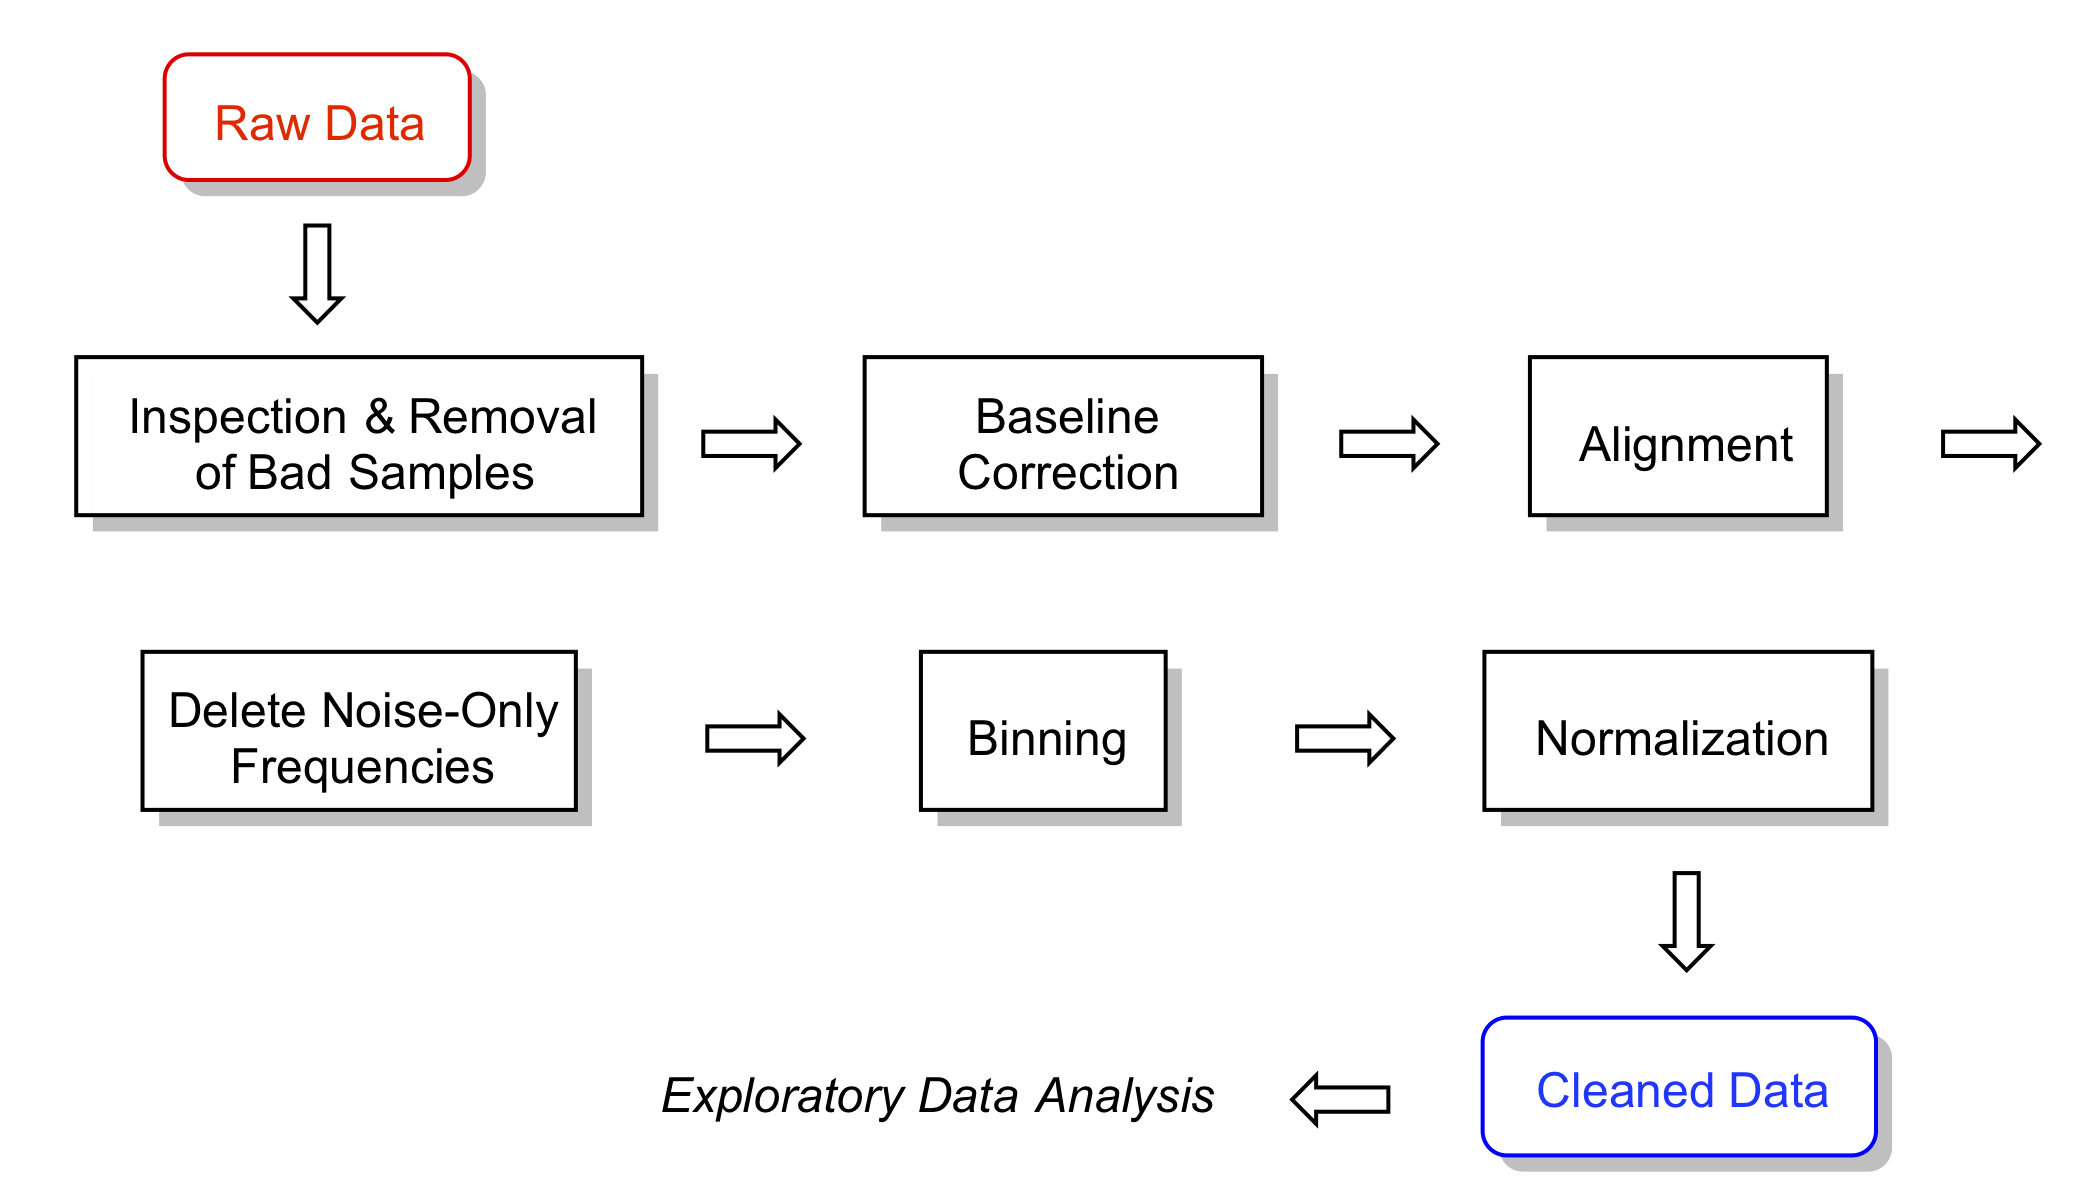
\includegraphics[scale = 1.0]{MetabPreProcess}
\caption{\label{WF}A typical workflow.  For a given data set, some steps may be omitted and the order changed.  That is part of what is meant by exploratory data analysis!}
\end{figure*}

\hypertarget{getting-data-into}{%
\section{\texorpdfstring{Getting Data into
\texttt{ChemoSpec}}{Getting Data into }}\label{getting-data-into}}

There are two means of importing raw data sets into \texttt{ChemoSpec}.
One is the function \texttt{files2SpectraObject}, which assumes that
your raw data exist as separate files in a single directory, each file
containing a frequency column and an intensity column. A header row may
or may not be present, and the data can be separated by any separation
mark you like (typically comma, tab, semi-colon or space). You may also
use comma or period as the decimal mark. These options permit data to be
imported from files written by a wide variety of instruments using
various
conventions.\footnote{My experience is that csv files don't always have comma as the separator, and of course conventions about decimal marks vary a bit around the world.  And an instrument installed in a certain country doesn't always follow local conventions.}
It is also possible to import files in the J-CAMP-DX format.

The second function is \texttt{matrix2SpectraObject}, which assumes you
have a single file containing a matrix of the data. This matrix should
have frequencies in the first column, and individual sample intensities
in the remaining columns. There must be a header row in the file, and it
must contain the sample names (except the first entry, which marks the
frequencies, is ignored). Other than this requirement, you have all the
flexibility described above.

Please be sure to read the help at \texttt{?files2SpectraObject} for the
details, and be certain to pay special attention to the \ldots argument,
as this is how your choice of header, separator, and decimal mark are
conveyed to \texttt{read.table} which does the actual reading.

It's a very good practice to name your data files using a system that
encodes any class membership. For example, if your data set contains
treatment and control groups, or any analogous class/group information,
this information should be available via the file names. The argument
\texttt{gr.crit} will be the basis for a grep process on the file/sample
names, and from there, each sample will be assigned to a group and be
assigned a color as well. If your samples don't fall into groups, that's
fine too, but you still have to give \texttt{gr.crit} something to go on
-- just give it one string that is common to all the file names.
Obviously, this approach encourages one to name the files as they come
off the instrument with forethought as to how they will be analyzed,
which in turn depends upon your experimental design. Nothing wrong with
having a plan!

The output of \texttt{files2SpectraObject} or
\texttt{matrix2SpectraObject} is a \texttt{Spectra} object, which is
\texttt{R}-speak for an object that contains not only your data, but
other information about the data, as provided by you via the arguments
to the function.

Here's a typical situation. Let's say you had a folder containing 30 NMR
files of flower essential oils. Imagine that 18 of these were from one
proposed subspecies, and 12 from another. Further, let's pretend that
the question under investigation has something to do with the taxonomy
of these two supposed subspecies, in other words, an investigation into
whether or not they should be considered subspecies at all. If the files
were named like \textcolor{blue}{sspA1.csv}
\ldots \textcolor{blue}{sspA18.csv} and \textcolor{blue}{sspB1.csv}
\ldots \textcolor{blue}{sspB12.csv} then the following command should
process the files and create the desired \texttt{Spectra} object:

\begin{Shaded}
\begin{Highlighting}[]
\NormalTok{ssp <{-}}\StringTok{ }\KeywordTok{files2SpectraObject}\NormalTok{(}
  \DataTypeTok{gr.crit =} \KeywordTok{c}\NormalTok{(}\StringTok{"sspA"}\NormalTok{, }\StringTok{"sspB"}\NormalTok{),}
  \DataTypeTok{gr.cols =} \KeywordTok{c}\NormalTok{(}\StringTok{"red"}\NormalTok{, }\StringTok{"blue"}\NormalTok{),}
  \DataTypeTok{freq.unit =} \StringTok{"ppm"}\NormalTok{,}
  \DataTypeTok{int.unit =} \StringTok{"peak intensity"}\NormalTok{,}
  \DataTypeTok{descrip =} \StringTok{"Subspecies Study"}\NormalTok{,}
  \DataTypeTok{out.file =} \StringTok{"subsp"}\NormalTok{)}
\end{Highlighting}
\end{Shaded}

This causes \texttt{files2SpectraObject} to inspect the file names for
the strings \texttt{"sspA"} and \texttt{"sspB"} and use these to assign
the samples into groups. Samples in \textcolor{blue}{sspA*.csv} files
will be assigned the color \texttt{red} and \textcolor{blue}{sspB*.csv}
will be assigned \texttt{blue} (see Section \ref{ColSym} for some
suggestions about planning ahead on color choices, as well as
\texttt{?colorSymbol}). After running this command, a new file called
\textcolor{blue}{subsp.RData} will be in your directory, and and a
\texttt{Spectra} object called \texttt{ssp} will be in your workspace
read for exploration. At a later date, you don't have to re-import your
data, you can use the saved version and give it whatever name you like
as follows (function \texttt{loadObject} is from package
\texttt{R.utils}):

\begin{Shaded}
\begin{Highlighting}[]
\NormalTok{SubspeciesNMR <{-}}\StringTok{ }\KeywordTok{loadObject}\NormalTok{(}\StringTok{"subsp.RData"}\NormalTok{)}
\end{Highlighting}
\end{Shaded}

Now it is ready to use.

\hypertarget{working-with-chromatograms}{%
\subsection{Working with
Chromatograms}\label{working-with-chromatograms}}

While all the language in this vignette and in the package are geared
toward analysis of spectra, \texttt{ChemoSpec} can also works quite well
with chromatograms as the raw data. In this case, time replaces
frequency of course, but other than that the analysis is virtually the
same. So the only real difference is when you import the data, e.g.~via
\texttt{files2SpectraObject}, you will give the frequency unit along
these lines: \texttt{freq.unit = "time (minutes)"}.

\hypertarget{built-in-data-sets}{%
\subsection{Built-in Data Sets}\label{built-in-data-sets}}

\texttt{ChemoSpec} ships with several built-in data sets.
\texttt{SrE.IR} is the set used for this vignette. It is composed of a
collection of 14 IR spectra of essential oil extracted from the palm
\emph{Serenoa repens} or Saw Palmetto, which is commonly used to treat
BPH in men. The 14 spectra are of different retail samples, and are
divided into two categories based upon the label description: adSrE,
adulterated extract, and pSrE, pure extract. The adulterated samples
typically have olive oil added to them, which has no effect on BPH.
There are two additional spectra included as references/outliers:
evening primrose oil, labeled EPO in the data set, and olive oil,
labeled OO. These latter two oils are mixtures of triglycerides for the
most part, while the SrE samples are largely fatty acids. As a result,
the spectra of these two groups differ: the glycerides have ester
carbonyl stretches and no O--H stretch, while the fatty acids have acid
carbonyl stretches and an O--H stretch consistent with a carboxylic acid
OH.

Also included is \texttt{SrE.NMR} which is the corresponding set of NMR
spectra, and \texttt{CuticleIR}. The latter is a series of IR spectra of
the cuticle (leaf surface) of the plant \emph{Portulaca oleracea}. The
data were taken by gently pinning the leaf against an ATR sampling
device. The plants were grown at two different temperatures, and two
different genotypes (varieties) were used (a classic G x E, genotype by
environment, experiment).

The \texttt{SrE.IR} data set is used as the example in this vignette as
the sample spectra are fairly different and give good separation by most
chemometric methods. The \texttt{CuticleIR} spectra differ in much more
subtle ways and as as result are more of a challenge to analyze. For
more details about these data sets, type \texttt{?data\_set\_name} at
the console.

\hypertarget{summarize-the-data}{%
\subsection{Summarize the Data}\label{summarize-the-data}}

\label{sec-prelim} \emph{The} first thing you should do, and this is
very important, is to make sure your data are in good shape. First, you
can summarize the data set you created, and verify that the data ranges
and other details look like you expect them to:

\begin{Shaded}
\begin{Highlighting}[]
\KeywordTok{data}\NormalTok{(SrE.IR) }\CommentTok{\# makes the data available}
\KeywordTok{sumSpectra}\NormalTok{(SrE.IR)}
\end{Highlighting}
\end{Shaded}

\begin{ShadedResult}
\begin{verbatim}
#  
#   Serenoa repens IR quality study 
#  
#   There are 16 spectra in this set.
#   The y-axis unit is absorbance.
#  
#   The frequency scale runs from
#   399.2123 to 3999.837 wavenumber
#   There are 1868 frequency values.
#   The frequency resolution is
#   1.9286 wavenumber/point.
#  
#  
#   The spectra are divided into 4 groups: 
#  
#    group no.   color symbol
#  1 adSrE  10 #984EA3     15
#  2   EPO   1 #377EB8      2
#  3    OO   1 #4DAF4A      3
#  4  pSrE   4 #E41A1C      1
#    alt.sym
#  1       d
#  2       b
#  3       c
#  4       a
#  
#  
#  *** Note: this is an S3 object
#  of class 'Spectra'
\end{verbatim}
\end{ShadedResult}

\texttt{sumSpectra} provides several pieces of information, and we'll
discuss some of them as we go along.

\hypertarget{plotting-the-spectra}{%
\section{Plotting the Spectra}\label{plotting-the-spectra}}

Assuming that everything looks good so far, it's time to plot the
spectra and inspect them. A good practice would be to check every
spectrum for artifacts and other potential problems. There are three
functions that can do this for you:

\begin{enumerate}
  \item \texttt{LoopThruSpectra} takes the pain out of inspecting quite a few spectra.  It shows you one spectrum at a time, and waits for a return to be typed in the console before proceeding.  See the help page for details.
  \item \texttt{plotSpectra} is intended for general use and publication-quality graphics.  You will generally have to play with the arguments a bit if plotting more than one spectrum.
  \item \texttt{plotSpectraJS} is the interactive version of \texttt{plotSpectra}.  It shows your data in a web page with the ability to offset the spectra and zoom as desired.  For really large data sets it may be slow; see the help page for ways to avoid that.
\end{enumerate}

A basic plot using \texttt{plotSpectra} is shown in Figure \ref{plot}.
In this case we have chosen to plot one spectrum from each category.
Note that the carbonyl and \(\mathsf{{C_{sp2}-H}}\) regions are clearly
different in these samples.

\begin{Shaded}
\begin{Highlighting}[]
\CommentTok{\# We\textquotesingle{}ll make a fancy title here}
\CommentTok{\# and re{-}use in other plots}
\NormalTok{myt <{-}}\StringTok{ }\KeywordTok{expression}\NormalTok{(}
  \KeywordTok{bolditalic}\NormalTok{(Serenoa)}\OperatorTok{\textasciitilde{}}
\StringTok{  }\KeywordTok{bolditalic}\NormalTok{(repens)}\OperatorTok{\textasciitilde{}}
\StringTok{  }\KeywordTok{bold}\NormalTok{(Extract}\OperatorTok{\textasciitilde{}}\NormalTok{IR}\OperatorTok{\textasciitilde{}}\NormalTok{Spectra))}
\KeywordTok{plotSpectra}\NormalTok{(SrE.IR,}
  \DataTypeTok{main =}\NormalTok{ myt,}
  \DataTypeTok{which =} \KeywordTok{c}\NormalTok{(}\DecValTok{1}\NormalTok{, }\DecValTok{2}\NormalTok{, }\DecValTok{14}\NormalTok{, }\DecValTok{16}\NormalTok{),}
  \DataTypeTok{yrange =} \KeywordTok{c}\NormalTok{(}\DecValTok{0}\NormalTok{, }\FloatTok{1.6}\NormalTok{),}
  \DataTypeTok{offset =} \FloatTok{0.4}\NormalTok{,}
  \DataTypeTok{lab.pos =} \DecValTok{2200}\NormalTok{)}
\end{Highlighting}
\end{Shaded}

\begin{figure}

{\centering 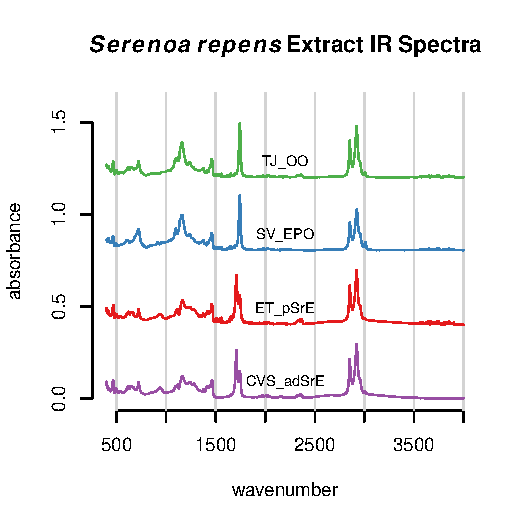
\includegraphics{/Users/bryanhanson/Documents/Professional/Research/R_Pkgs/ChemoSpec/docs/articles/ChemoSpec_files/figure-latex/Chunk8-1} 

}

\caption{\label{plot}Sample plot.}\label{fig:Chunk8}
\end{figure}

Depending upon the intensity range of your data set, and the number of
spectra to be plotted, you have to manually adjust the arguments
\texttt{yrange}, \texttt{offset} and \texttt{amplify}, but this usually
only takes a few iterations. Keep in mind that \texttt{offset}, and
\texttt{amplify} are multiplied in the function, so if you increase one,
you may need to decrease the other. Suppose that you wanted to focus
just on the carbonyl region of these spectra; you can add the argument
\texttt{xlim}. To demonstrate, let's look at fewer spectra, and at
higher amplitude, so we can see details, as shown in Figure
\ref{subplot}.

\begin{Shaded}
\begin{Highlighting}[]
\KeywordTok{plotSpectra}\NormalTok{(SrE.IR,}
  \DataTypeTok{main =}\NormalTok{ myt,}
  \DataTypeTok{which =} \KeywordTok{c}\NormalTok{(}\DecValTok{1}\NormalTok{, }\DecValTok{2}\NormalTok{, }\DecValTok{14}\NormalTok{, }\DecValTok{16}\NormalTok{),}
  \DataTypeTok{yrange =} \KeywordTok{c}\NormalTok{(}\DecValTok{0}\NormalTok{, }\FloatTok{0.6}\NormalTok{),}
  \DataTypeTok{offset =} \FloatTok{0.1}\NormalTok{,}
  \DataTypeTok{lab.pos =} \DecValTok{1775}\NormalTok{,}
  \DataTypeTok{xlim =} \KeywordTok{c}\NormalTok{(}\DecValTok{1650}\NormalTok{, }\DecValTok{1800}\NormalTok{))}
\end{Highlighting}
\end{Shaded}

\begin{figure}

{\centering 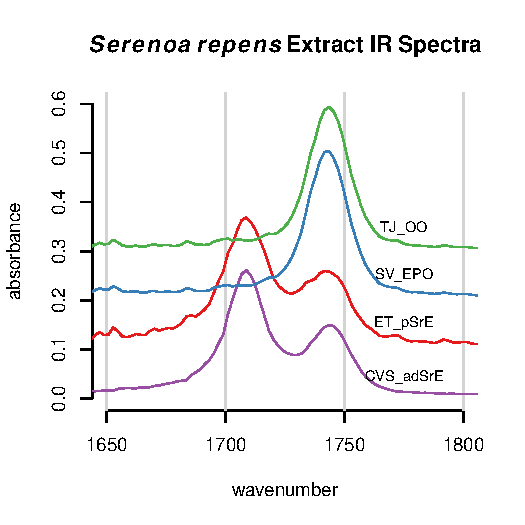
\includegraphics{/Users/bryanhanson/Documents/Professional/Research/R_Pkgs/ChemoSpec/docs/articles/ChemoSpec_files/figure-latex/Chunk10-1} 

}

\caption{\label{subplot}Detail of the carbonyl region.}\label{fig:Chunk10}
\end{figure}

These sample plots display the IR spectra in two ways that may be
upsetting to some readers: First, the x-axis is ``backwards'', because
the underlying spectra were originally saved with an ascending frequency
axis (which is not always the case). This is readily fixed by supplying
the \texttt{xlim} argument in the desired order,
e.g.~\texttt{xlim = c(1800, 1650)} in the previous example. Second, the
vertical scale in these examples is absorbance. When using IR for
structural elucidation, the vertical axis is typically \%T, with the
peaks pointing downward. However, absorbance mode is the appropriate one
for chemometrics. Record your original spectra that way and get used to
it.

The argument \texttt{which} in \texttt{plotSpectra} takes a integer
vector of the spectra you wish to plot--- you can think of this as the
row number if you imagine each spectra to be a row in a matrix, with
intensities in the columns (with each column corresponding to a
particular frequency value). You may be wondering how to determine which
particular sample is in each row. This is best accomplished with a grep
command. For instance, if you wanted to know what row/sample the olive
oil was in, either of the following methods would locate it for you:

\begin{Shaded}
\begin{Highlighting}[]
\CommentTok{\# if there are only a few spectra}
\CommentTok{\# show all of the names}
\NormalTok{SrE.IR}\OperatorTok{$}\NormalTok{names}
\end{Highlighting}
\end{Shaded}

\begin{ShadedResult}
\begin{verbatim}
#   [1] "CVS_adSrE" "ET_pSrE"  
#   [3] "GNC_adSrE" "LF_adSrE" 
#   [5] "MDB_pSrE"  "NA_pSrE"  
#   [7] "Nat_adSrE" "NP_adSrE" 
#   [9] "NR_pSrE"   "NSI_adSrE"
#  [11] "NW_adSrE"  "SN_adSrE" 
#  [13] "Sol_adSrE" "SV_EPO"   
#  [15] "TD_adSrE"  "TJ_OO"
\end{verbatim}
\end{ShadedResult}

\begin{Shaded}
\begin{Highlighting}[]
\CommentTok{\# if there are a lot of spectra,}
\CommentTok{\# grep for the desired names}
\KeywordTok{grep}\NormalTok{(}\StringTok{"OO"}\NormalTok{, SrE.IR}\OperatorTok{$}\NormalTok{names)}
\end{Highlighting}
\end{Shaded}

\begin{ShadedResult}
\begin{verbatim}
#  [1] 16
\end{verbatim}
\end{ShadedResult}

\hypertarget{data-pre-processing-options}{%
\section{Data Pre-Processing
Options}\label{data-pre-processing-options}}

There are a number of data pre-processing options available for your
consideration. The main choices are whether to normalize the data,
whether to bin the data, and whether to scale the data. Baseline
correction is another typical action, and for some NMR data sets one
might need to carry out aligment. Data scaling is handled by the PCA
routines, see Section \ref{sec-pca}. \cite{Engel2013} has a good
discussion of pre-processing. \cite{Karakach2009} has a good discussion
of error sources in \(\mathsf{^{1}H}\) NMR data.

\hypertarget{correcting-baseline-drift}{%
\subsection{Correcting Baseline Drift}\label{correcting-baseline-drift}}

\texttt{ChemoSpec} uses the functions in the package \texttt{baseline}
to correct wandering baselines. The function, \texttt{baselineSpectra},
can show you the original and corrected baselines if desired, which is
useful for choosing a method. Figure \ref{baseline} shows a typical
usage. Method \texttt{rfbaseline} works well for IR spectra;
\texttt{retC = TRUE} puts the corrected spectra into the new
\texttt{Spectra} object so we can use it going forward (and we will).

\begin{Shaded}
\begin{Highlighting}[]
\NormalTok{SrE2.IR <{-}}\StringTok{ }\KeywordTok{baselineSpectra}\NormalTok{(SrE.IR,}
  \DataTypeTok{int =} \OtherTok{FALSE}\NormalTok{,}
  \DataTypeTok{method =} \StringTok{"modpolyfit"}\NormalTok{,}
  \DataTypeTok{retC =} \OtherTok{TRUE}\NormalTok{)}
\end{Highlighting}
\end{Shaded}

\begin{figure}

{\centering 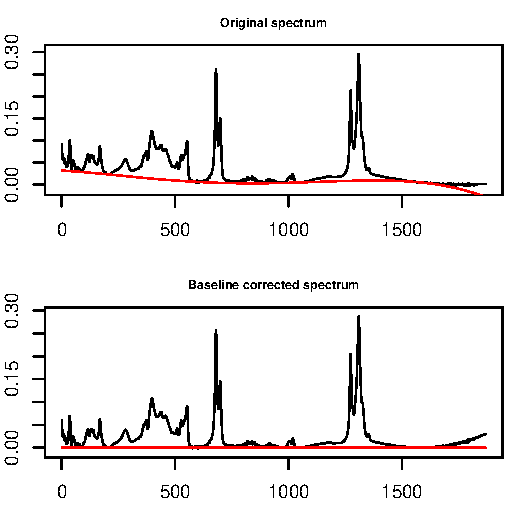
\includegraphics{/Users/bryanhanson/Documents/Professional/Research/R_Pkgs/ChemoSpec/docs/articles/ChemoSpec_files/figure-latex/Chunk10b-1} 

}

\caption{\label{baseline}Correcting baseline drift.}\label{fig:Chunk10b}
\end{figure}

\hypertarget{alignment}{%
\subsection{Alignment}\label{alignment}}

For \(\mathsf{^{1}H}\) NMR data, it is sometimes desirable to align the
spectra. This compensates in part for changes in dilution, ionic
strength, or pH that can cause significant shifts for some types of
protons. Spectra with broad, rolling peaks won't have this problem
(UV-Vis or IR for example). \texttt{ChemoSpec} provides the
\texttt{clupaSpectra} for this purpose. You can see an example
\href{http://www.validnmr.com/w/index.php?title=Chemometrics}{here}.

\hypertarget{bucketing-or-binning}{%
\subsection{Bucketing or Binning}\label{bucketing-or-binning}}

Another type of pre-processing that you may wish to consider is binning
or bucketing, in which groups of frequencies are collapsed into one
frequency value, and the corresponding intensities are summed. There are
two reasons for doing this:

\begin{enumerate}
  \item Compacting large data sets:  This is a historical issue, the algorithms in \texttt{R} are quite fast, and large data sets don't really slow it down much.
  \item  Compensating for $\mathsf{^{1}H}$ NMR shifts, as described above.
\end{enumerate}

This example illustrates the process but is not necessary with IR data:

\begin{Shaded}
\begin{Highlighting}[]
\NormalTok{tmp <{-}}\StringTok{ }\KeywordTok{binSpectra}\NormalTok{(SrE.IR, }\DataTypeTok{bin.ratio =} \DecValTok{4}\NormalTok{)}
\KeywordTok{sumSpectra}\NormalTok{(tmp)}
\end{Highlighting}
\end{Shaded}

\begin{ShadedResult}
\begin{verbatim}
#  
#   Serenoa repens IR quality study 
#  
#   There are 16 spectra in this set.
#   The y-axis unit is absorbance.
#  
#   The frequency scale runs from
#   402.1052 to 3996.945 wavenumber
#   There are 467 frequency values.
#   The frequency resolution is
#   7.71425 wavenumber/point.
#  
#  
#   The spectra are divided into 4 groups: 
#  
#    group no.   color symbol
#  1 adSrE  10 #984EA3     15
#  2   EPO   1 #377EB8      2
#  3    OO   1 #4DAF4A      3
#  4  pSrE   4 #E41A1C      1
#    alt.sym
#  1       d
#  2       b
#  3       c
#  4       a
#  
#  
#  *** Note: this is an S3 object
#  of class 'Spectra'
\end{verbatim}
\end{ShadedResult}

Compare the results here with the \texttt{sumSpectra} of the full data
set (Section \ref{sec-prelim}). In particular note that the frequency
resolution has gone down due to the binning process. \texttt{ChemoSpec}
uses the simplest of binning algorithms: after perhaps dropping a few
points (with a warning) to make your data set divisible by the specified
\texttt{bin.ratio}, data points are replaced by the average frequency
and the sum of the grouped intensities. Depending upon the fine
structure in your data and the \texttt{bin.ratio} this might cause
important peaks to be split between different bins. There are more
sophisticated binning algorithms in the literature that try to address
this, but none are currently implemented in \texttt{ChemoSpec}
\citep{Anderson2008, DeMeyer2008, Sousa2013}. It's probably better to
align the spectra as described above.

\hypertarget{normalization}{%
\subsection{Normalization}\label{normalization}}

Normalization is handled by the \texttt{normSpectra} function. Usually
one normalizes data in which the sample preparation procedure may lead
to differences in concentration, such as body fluids that might have
been diluted during handling, or that vary due to the physiological
state of the organism studied. The \texttt{SrE.IR} data set is taken by
placing the oil extract directly on an ATR device and no dilution is
possible, so normalization isn't really appropriate. Please see the help
page for the normalization options. The literature contains a number of
useful discussions about normalization
issues.\citep{Craig2006, Romano2000, vandenBerg2006, Filzmoser2009, Zhang2009}

\hypertarget{editing-the-data-set-spectral-regions}{%
\section{Editing the Data Set \& Spectral
Regions}\label{editing-the-data-set-spectral-regions}}

In the process of plotting and inspecting your spectra, you may find
some spectra/samples that have problems. Perhaps they have instrumental
artifacts. Or maybe you have decided to eliminate one subgroup of
samples from your data set to see how the results differ.

\hypertarget{removing-individual-samples}{%
\subsection{Removing Individual
Samples}\label{removing-individual-samples}}

To remove a particular sample, or samples meeting a certain criteria,
you use the \texttt{removeSample} function. This function uses a
grepping process based on its \texttt{rem.sam} argument, so you must be
careful due to the greediness of grep. Let's imagine that sample
TD\_adSrE has artifacts and needs to be removed. The command would be:

\begin{Shaded}
\begin{Highlighting}[]
\NormalTok{noTD <{-}}\StringTok{ }\KeywordTok{removeSample}\NormalTok{(SrE2.IR,}
  \DataTypeTok{rem.sam =} \KeywordTok{c}\NormalTok{(}\StringTok{"TD\_adSrE"}\NormalTok{))}
\KeywordTok{sumSpectra}\NormalTok{(noTD)}
\end{Highlighting}
\end{Shaded}

\begin{ShadedResult}
\begin{verbatim}
#  
#   Serenoa repens IR quality study 
#  
#   There are 15 spectra in this set.
#   The y-axis unit is absorbance.
#  
#   The frequency scale runs from
#   399.2123 to 3999.837 wavenumber
#   There are 1868 frequency values.
#   The frequency resolution is
#   1.9286 wavenumber/point.
#  
#  
#   The spectra are divided into 4 groups: 
#  
#    group no.   color symbol
#  1 adSrE   9 #984EA3     15
#  2   EPO   1 #377EB8      2
#  3    OO   1 #4DAF4A      3
#  4  pSrE   4 #E41A1C      1
#    alt.sym
#  1       d
#  2       b
#  3       c
#  4       a
#  
#  
#  *** Note: this is an S3 object
#  of class 'Spectra'
\end{verbatim}
\end{ShadedResult}

\begin{Shaded}
\begin{Highlighting}[]
\KeywordTok{grep}\NormalTok{(}\StringTok{"TD\_adSrE"}\NormalTok{, noTD}\OperatorTok{$}\NormalTok{names)}
\end{Highlighting}
\end{Shaded}

\begin{ShadedResult}
\begin{verbatim}
#  integer(0)
\end{verbatim}
\end{ShadedResult}

The \texttt{sumSpectra} command confirms that there are now one fewer
spectra in the set. As shown, you could also re-grep for the sample name
to verify that it is not found. The first argument in \texttt{grep} is
the pattern you are searching for; if that pattern matches more than one
name they will all be ``caught.'' For example if you used ``SrE'' as
your pattern you would remove all the samples except the two reference
samples, since ``SrE'' occurs in ``adSrE'' and ``pSrE''. You can check
this in advance with the grep function itself:

\begin{Shaded}
\begin{Highlighting}[]
\NormalTok{SrE <{-}}\StringTok{ }\KeywordTok{grep}\NormalTok{(}\StringTok{"SrE"}\NormalTok{, SrE2.IR}\OperatorTok{$}\NormalTok{names)}
\CommentTok{\# show the name(s) that contain "SrE"}
\NormalTok{SrE2.IR}\OperatorTok{$}\NormalTok{names[SrE]}
\end{Highlighting}
\end{Shaded}

\begin{ShadedResult}
\begin{verbatim}
#   [1] "CVS_adSrE" "ET_pSrE"  
#   [3] "GNC_adSrE" "LF_adSrE" 
#   [5] "MDB_pSrE"  "NA_pSrE"  
#   [7] "Nat_adSrE" "NP_adSrE" 
#   [9] "NR_pSrE"   "NSI_adSrE"
#  [11] "NW_adSrE"  "SN_adSrE" 
#  [13] "Sol_adSrE" "TD_adSrE"
\end{verbatim}
\end{ShadedResult}

\begin{Shaded}
\begin{Highlighting}[]
\NormalTok{SrE }\CommentTok{\# gives the corresponding indices}
\end{Highlighting}
\end{Shaded}

\begin{ShadedResult}
\begin{verbatim}
#   [1]  1  2  3  4  5  6  7  8
#   [9]  9 10 11 12 13 15
\end{verbatim}
\end{ShadedResult}

This is what is meant by ``grep is greedy''. In this situation, you have
three choices:

\begin{enumerate}
  \item You could manually remove the problem samples (\texttt{str(SrE2.IR)}) would give you an idea of how to do that; see also below under Hierarchical Cluster Analysis).
  \item \texttt{removeSample} also accepts indices of samples, so you could grep as above, note the index of the sample you actually want to remove, and use that in \texttt{rem.sam}.
  \item If you know a bit about grep and regular expressions, you can pass a more sophisticated search pattern to \texttt{rem.sam}.
\end{enumerate}

\hypertarget{removing-groups}{%
\subsection{Removing Groups}\label{removing-groups}}

\texttt{removeSample} uses the names of the samples (in
\texttt{Spectra\$names}) to identify and remove individual samples from
the \texttt{Spectra} object. There is also a function
\texttt{removeGroup} which will remove samples belonging to a particular
group in \texttt{Spectra\$groups}.

\hypertarget{identifying-removing-frequencies-of-no-interest}{%
\subsection{Identifying \& Removing Frequencies of No
Interest}\label{identifying-removing-frequencies-of-no-interest}}

Many spectra will have regions that should be removed before analysis.
It may be an uninformative, interfering peak like the water peak in
\(\mathsf{^{1}H}\) NMR, or the \(\mathsf{CO_2}\) peak in IR. Or, there
may be regions of the spectra that simply don't have much information --
they contribute a noisy baseline and not much else. An example would be
the region from about 1,800 or 1,900 \(\mathsf{cm^{-1}}\) to about 2,500
\(\mathsf{cm^{-1}}\) in IR, a region where there are typically no peaks
except for the atmospheric \(\mathsf{CO_2}\) stretch, and rarely (be
careful!) alkyne stretches.

Finding these regions might be pretty simple, a matter of inspection
coupled with your knowledge of spectroscopy. Another approach is to use
the function \texttt{surveySpectra} to examine the entire set of
spectra. This function computes a summary statistic (your choice) of the
intensities at a particular frequency across the data set, as well as
the mean or median. In regions with little variation, the mean/median
and upper/lower summary lines will be close together. Figure \ref{surv}
demonstrates the process. There is also an alternative,
\texttt{surveySpectra2} which presents the data in a slightly different
format. See Figure \ref{surv2}.

\begin{Shaded}
\begin{Highlighting}[]
\KeywordTok{surveySpectra}\NormalTok{(SrE2.IR,}
  \DataTypeTok{method =} \StringTok{"iqr"}\NormalTok{,}
  \DataTypeTok{main =}\NormalTok{ myt,}
  \DataTypeTok{by.gr =} \OtherTok{FALSE}\NormalTok{)}
\end{Highlighting}
\end{Shaded}

\begin{figure}

{\centering 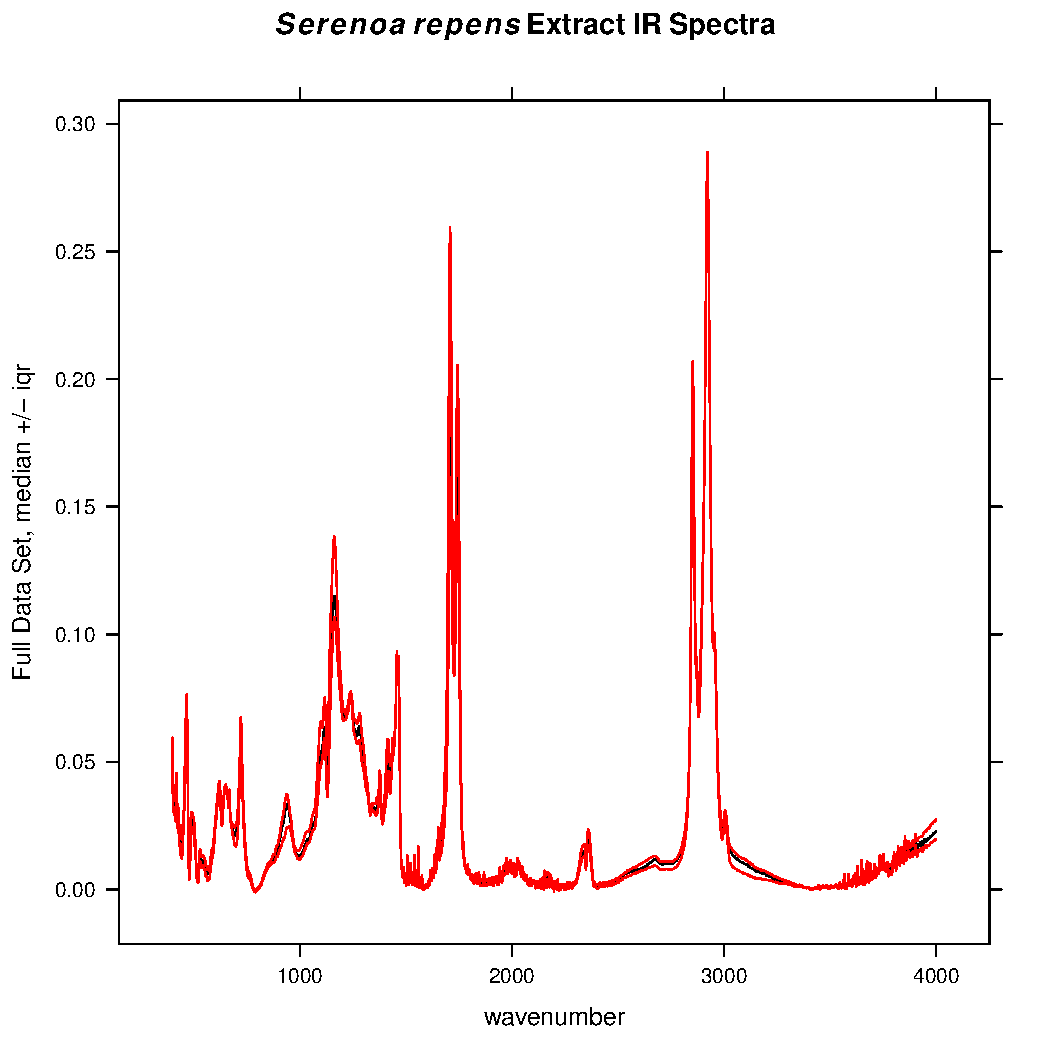
\includegraphics[width=\linewidth,height=\linewidth]{/Users/bryanhanson/Documents/Professional/Research/R_Pkgs/ChemoSpec/docs/articles/ChemoSpec_files/figure-latex/Chunk14-1} 

}

\caption{\label{surv}Checking for regions of no interest.}\label{fig:Chunk14}
\end{figure}

\begin{Shaded}
\begin{Highlighting}[]
\KeywordTok{surveySpectra2}\NormalTok{(SrE2.IR,}
  \DataTypeTok{method =} \StringTok{"iqr"}\NormalTok{,}
  \DataTypeTok{main =}\NormalTok{ myt)}
\end{Highlighting}
\end{Shaded}

\begin{figure}

{\centering 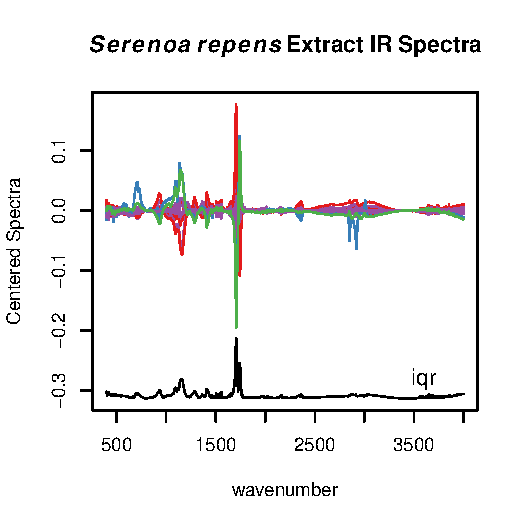
\includegraphics{/Users/bryanhanson/Documents/Professional/Research/R_Pkgs/ChemoSpec/docs/articles/ChemoSpec_files/figure-latex/Chunk14d-1} 

}

\caption{\label{surv2}Checking for regions of no interest.}\label{fig:Chunk14d}
\end{figure}

In Figure \ref{surv} we kept all the groups together by using argument
\texttt{by.gr = FALSE}. We also looked at the entire spectral range. In
Figure \ref{survA} we can look just at the carbonyl region. The black
line is the median value of intensity across the entire set of spectra.
The red lines are the upper and lower interquartile ranges which makes
it pretty clear that the carbonyl region of this data set varies a
lot.\footnote{A few plots in this vignette use smaller fonts; this is an artifact of using a two-column format and does not occur when creating full size plots.}

\begin{Shaded}
\begin{Highlighting}[]
\KeywordTok{surveySpectra}\NormalTok{(SrE2.IR,}
  \DataTypeTok{method =} \StringTok{"iqr"}\NormalTok{,}
  \DataTypeTok{main =} \StringTok{"Detail of Carbonyl Region"}\NormalTok{,}
  \DataTypeTok{by.gr =} \OtherTok{FALSE}\NormalTok{,}
  \DataTypeTok{xlim =} \KeywordTok{c}\NormalTok{(}\DecValTok{1650}\NormalTok{, }\DecValTok{1800}\NormalTok{))}
\end{Highlighting}
\end{Shaded}

\begin{figure}

{\centering 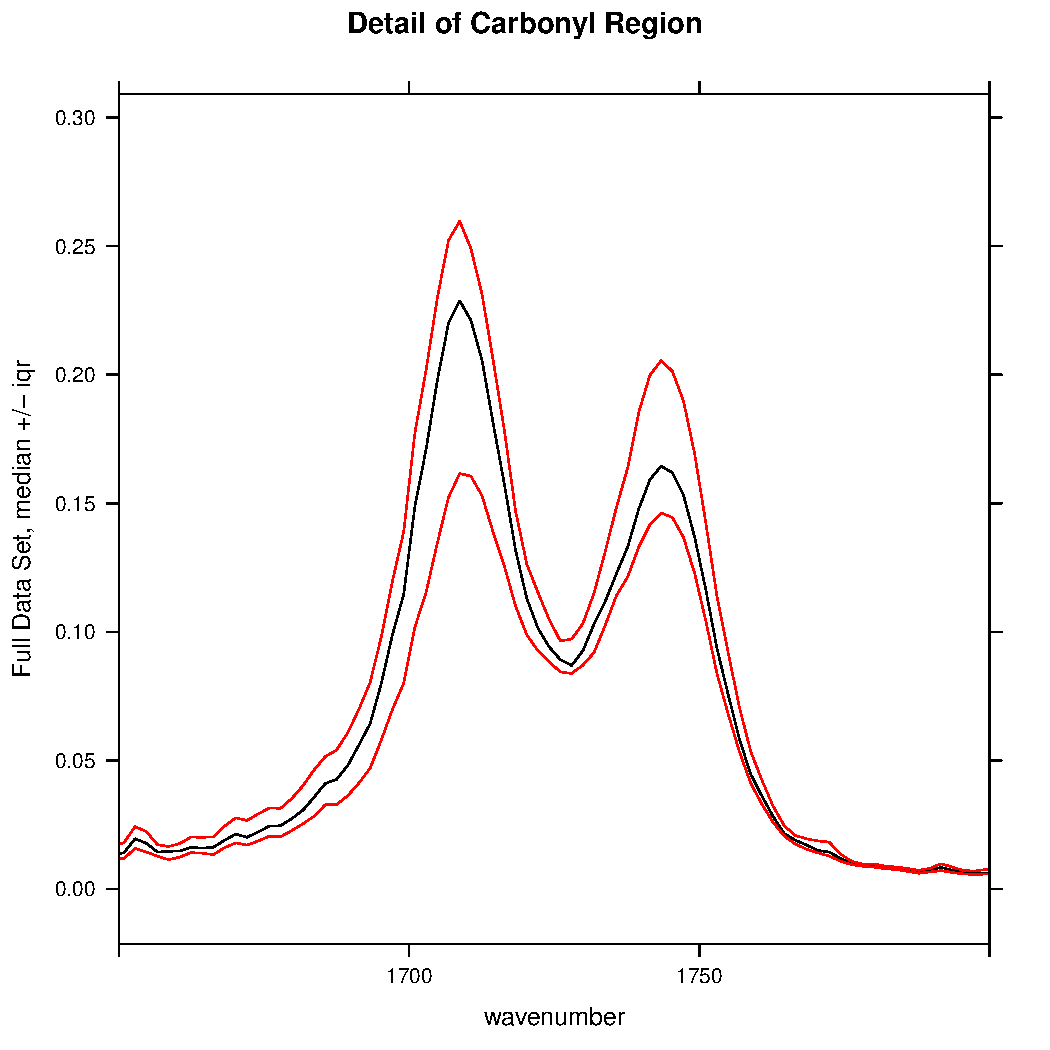
\includegraphics[width=\linewidth,height=\linewidth]{/Users/bryanhanson/Documents/Professional/Research/R_Pkgs/ChemoSpec/docs/articles/ChemoSpec_files/figure-latex/Chunk14a-1} 

}

\caption{\label{survA}Detail of carbonyl region.}\label{fig:Chunk14a}
\end{figure}

Finally, \texttt{surveySpectra} allows us to view the data set by group,
which is really more useful. Let's look at the carbonyl region by group
(Figure \ref{survB}). Note that we get warnings because two of the
groups have too few members to compute the interquartile range, and
these are not shown.

\begin{Shaded}
\begin{Highlighting}[]
\KeywordTok{surveySpectra}\NormalTok{(SrE2.IR,}
  \DataTypeTok{method =} \StringTok{"iqr"}\NormalTok{,}
  \DataTypeTok{main =} \StringTok{"Detail of Carbonyl Region"}\NormalTok{,}
  \DataTypeTok{by.gr =} \OtherTok{TRUE}\NormalTok{,}
  \DataTypeTok{xlim =} \KeywordTok{c}\NormalTok{(}\DecValTok{1650}\NormalTok{, }\DecValTok{1800}\NormalTok{))}
\end{Highlighting}
\end{Shaded}

\begin{ShadedResult}
\begin{verbatim}
#  
#  Group EPO has 3 or fewer members
#   so your stats are not very useful...
#   This group has been dropped for display purposes!
\end{verbatim}
\end{ShadedResult}
\begin{ShadedResult}
\begin{verbatim}
#  
#  Group OO has 3 or fewer members
#   so your stats are not very useful...
#   This group has been dropped for display purposes!
\end{verbatim}
\end{ShadedResult}
\begin{figure}

{\centering 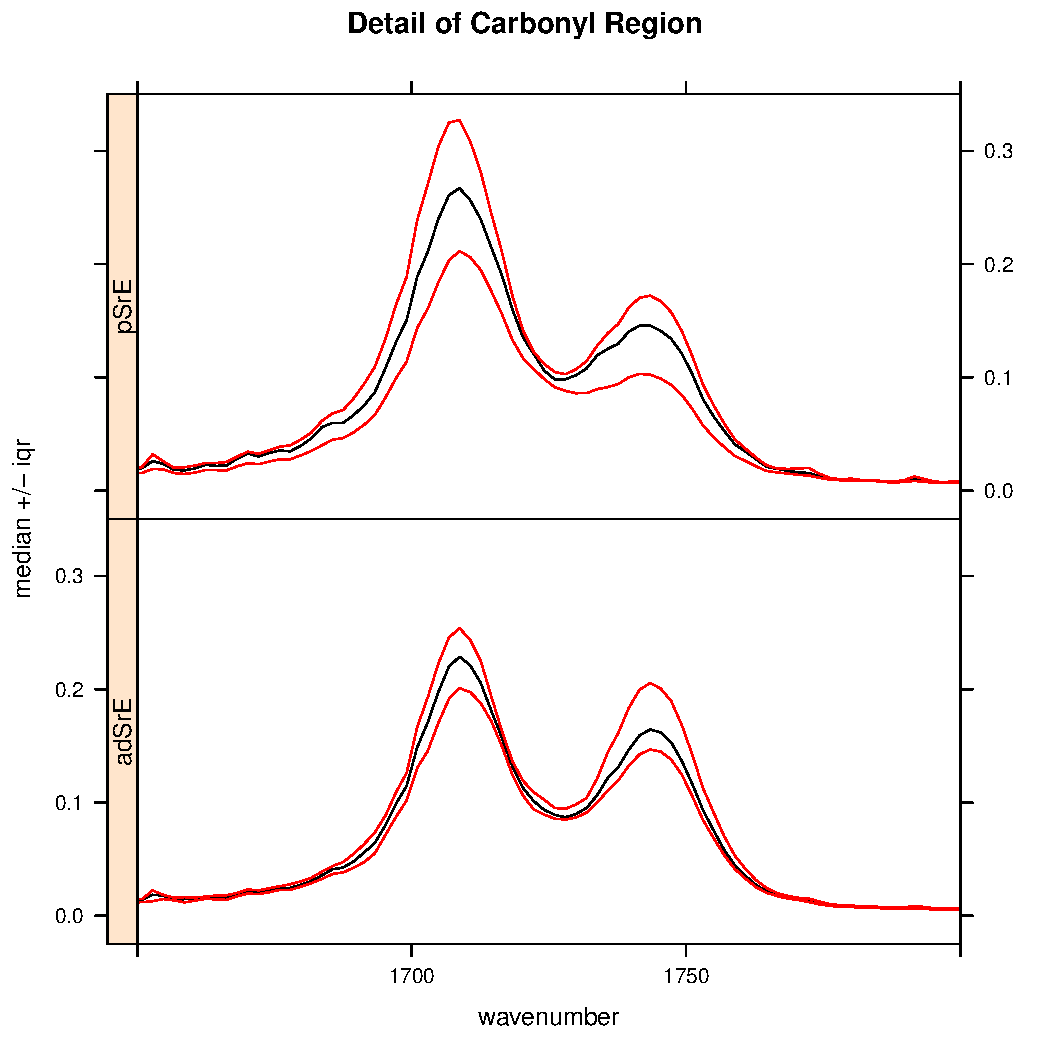
\includegraphics[width=\linewidth,height=\linewidth]{/Users/bryanhanson/Documents/Professional/Research/R_Pkgs/ChemoSpec/docs/articles/ChemoSpec_files/figure-latex/Chunk14b-1} 

}

\caption{\label{survB}Detail of carbonyl region by group.}\label{fig:Chunk14b}
\end{figure}

For reasons that will become evident in a moment, let's look at the
region between 1800 and 2500 \(\mathsf{cm^{-1}}\) (Figure \ref{survC}).

\begin{Shaded}
\begin{Highlighting}[]
\KeywordTok{surveySpectra}\NormalTok{(SrE2.IR,}
  \DataTypeTok{method =} \StringTok{"iqr"}\NormalTok{,}
  \DataTypeTok{main =} \StringTok{"Detail of Empty Region"}\NormalTok{,}
  \DataTypeTok{by.gr =} \OtherTok{FALSE}\NormalTok{,}
  \DataTypeTok{xlim =} \KeywordTok{c}\NormalTok{(}\DecValTok{1800}\NormalTok{, }\DecValTok{2500}\NormalTok{),}
  \DataTypeTok{ylim =} \KeywordTok{c}\NormalTok{(}\FloatTok{0.0}\NormalTok{, }\FloatTok{0.05}\NormalTok{))}
\end{Highlighting}
\end{Shaded}

\begin{figure}

{\centering 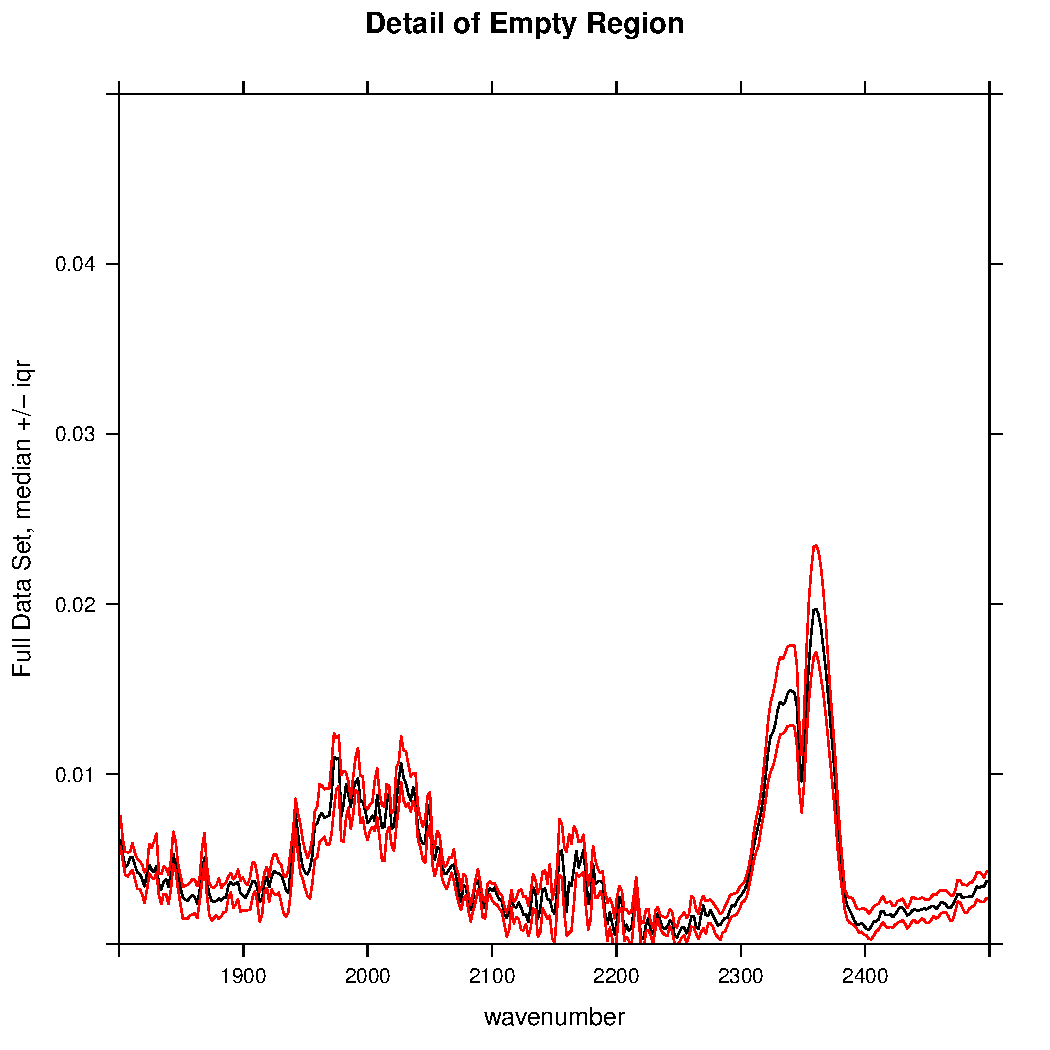
\includegraphics[width=\linewidth,height=\linewidth]{/Users/bryanhanson/Documents/Professional/Research/R_Pkgs/ChemoSpec/docs/articles/ChemoSpec_files/figure-latex/Chunk14c-1} 

}

\caption{\label{survC}Inspection of an uninteresting spectral region.}\label{fig:Chunk14c}
\end{figure}

From a theoretical perspective, we expect this region to be devoid of
interesting peaks. In fact, even when pooling the groups the signal in
this region is very weak, and the only peak present is due to
atmospheric \(\mathsf{CO_2}\). We can remove this region, since it is
primarily noise and artifact, with the function \texttt{removeFreq} as
follows. Note that there are fewer frequency points now.

\begin{Shaded}
\begin{Highlighting}[]
\NormalTok{SrE3.IR <{-}}\StringTok{ }\KeywordTok{removeFreq}\NormalTok{(SrE2.IR,}
  \DataTypeTok{rem.freq =}\NormalTok{ SrE2.IR}\OperatorTok{$}\NormalTok{freq }\OperatorTok{>}\StringTok{ }\DecValTok{1800} \OperatorTok{\&}
\StringTok{  }\NormalTok{SrE2.IR}\OperatorTok{$}\NormalTok{freq }\OperatorTok{<}\StringTok{ }\DecValTok{2500}\NormalTok{)}
\KeywordTok{sumSpectra}\NormalTok{(SrE3.IR)}
\end{Highlighting}
\end{Shaded}

\begin{ShadedResult}
\begin{verbatim}
#  
#   Serenoa repens IR quality study 
#  
#   There are 16 spectra in this set.
#   The y-axis unit is absorbance.
#  
#   The frequency scale runs from
#   399.2123 to 3999.837 wavenumber
#   There are 1505 frequency values.
#   The frequency resolution is
#   1.9286 wavenumber/point.
#  
#   This data set is not continuous
#   along the frequency axis.
#   Here are the data chunks:
#  
#     beg.freq end.freq     size
#  1  399.2123 1799.348 1400.136
#  2 2501.3450 3999.837 1498.492
#    beg.indx end.indx
#  1        1      727
#  2      728     1505
#  
#   The spectra are divided into 4 groups: 
#  
#    group no.   color symbol
#  1 adSrE  10 #984EA3     15
#  2   EPO   1 #377EB8      2
#  3    OO   1 #4DAF4A      3
#  4  pSrE   4 #E41A1C      1
#    alt.sym
#  1       d
#  2       b
#  3       c
#  4       a
#  
#  
#  *** Note: this is an S3 object
#  of class 'Spectra'
\end{verbatim}
\end{ShadedResult}

Notice that \texttt{sumSpectra} has identified a gap in the data set.
You can see this gap in the data as shown in Figure \ref{gaps}
(\texttt{sumSpectra} checks for gaps, but doesn't produce the plot);
both the numerical results and a figure are provided.

\begin{Shaded}
\begin{Highlighting}[]
\KeywordTok{check4Gaps}\NormalTok{(SrE3.IR}\OperatorTok{$}\NormalTok{freq, SrE3.IR}\OperatorTok{$}\NormalTok{data[}\DecValTok{1}\NormalTok{,])}
\end{Highlighting}
\end{Shaded}

\begin{figure}

{\centering 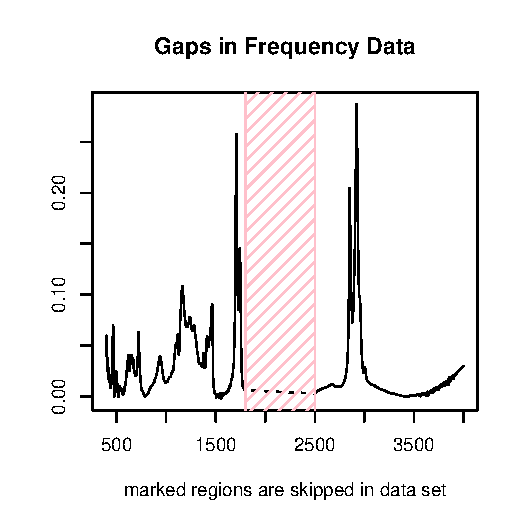
\includegraphics{/Users/bryanhanson/Documents/Professional/Research/R_Pkgs/ChemoSpec/docs/articles/ChemoSpec_files/figure-latex/Chunk7-1} 

}

\caption{\label{gaps}Identifying gaps in a data set.}\label{fig:Chunk7}
\end{figure}
\begin{ShadedResult}
\begin{verbatim}
#     beg.freq end.freq     size
#  1  399.2123 1799.348 1400.136
#  2 2501.3450 3999.837 1498.492
#    beg.indx end.indx
#  1        1      727
#  2      728     1505
\end{verbatim}
\end{ShadedResult}

\hypertarget{exploratory-data-analysis}{%
\section{Exploratory Data Analysis}\label{exploratory-data-analysis}}

\hypertarget{hierarchical-cluster-analysis}{%
\subsection{Hierarchical Cluster
Analysis}\label{hierarchical-cluster-analysis}}

\label{sec-hca} Hierarchical cluster analysis (HCA from now on) is a
clustering method (no surprise!) in which ``distances'' between samples
are calculated and displayed in a dendrogram (a tree-like structure;
these are also used in evolution and systematics where they are called
cladograms). The details behind HCA can be readily found elsewhere
(Chapter 6 of \cite{Filzmoser2009} is a good choice). With
\texttt{ChemoSpec} you have access to any of the methods available for
computing distances between samples and any of the methods for
identifying clusters. A typical example is shown in Figure \ref{hca}.

\begin{Shaded}
\begin{Highlighting}[]
\NormalTok{HCA <{-}}\StringTok{ }\KeywordTok{hcaSpectra}\NormalTok{(SrE3.IR, }\DataTypeTok{main =}\NormalTok{ myt)}
\end{Highlighting}
\end{Shaded}

\begin{figure}

{\centering 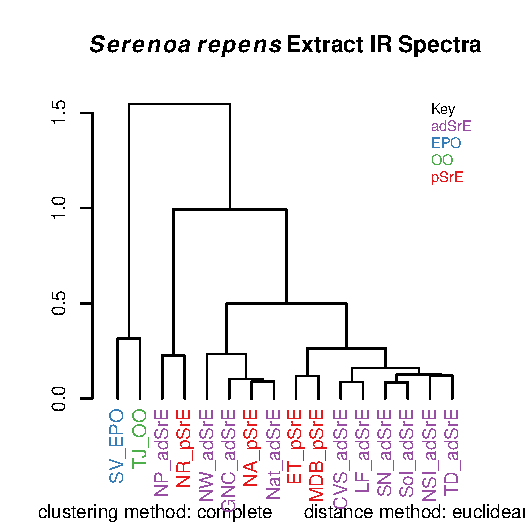
\includegraphics{/Users/bryanhanson/Documents/Professional/Research/R_Pkgs/ChemoSpec/docs/articles/ChemoSpec_files/figure-latex/Chunk19-1} 

}

\caption{\label{hca}Hierarchical cluster analysis.}\label{fig:Chunk19}
\end{figure}

The result is a dendrogram. The vertical scale represents the numerical
distance between samples. Not unexpectedly, the two reference samples
which are known to be chemically different cluster together separately
from all other samples. Perhaps surprisingly, the various pure and
adulterated oil extracts do not group together precisely. The function
\texttt{hcaScores} does the same kind of analysis using the results of
PCA, rather than the raw spectra. It is discussed in the next section.

\hypertarget{principal-components-analysis}{%
\subsection{Principal Components
Analysis}\label{principal-components-analysis}}

\label{sec-pca} Principal components analysis (PCA from now on) is the
real workhorse of exploratory data analysis. It makes no assumptions
about group membership, but clustering of the resulting sample scores
can be very helpful in understanding your data. The theory and practice
of PCA is covered well elsewhere (Chapter 3 of \cite{Filzmoser2009} is
an excellent choice). Here, we'll concentrate on using the PCA methods
in \texttt{ChemoSpec}. Briefly however, you can think of PCA as
determining the minimum number of components necessary to describe a
data set, in effect, removing noise and redundant information. Think of
a typical spectrum: some regions are clearly just noise. Further, a
typical spectroscopic peak spans quite a few frequency units as the peak
goes up, tops out, and then returns to baseline. Any one of the points
in a particular peak describe much the same thing, namely the intensity
of the peak. Plus, each frequency within a given peak envelope is
correlated to every other frequency in the envelope (they rise and fall
in unison as the peak changes size from sample to sample). PCA can look
``past'' all the noise and underlying correlation in the data set, and
boil the entire data set down to essentials. Unfortunately, the
principal components that are uncovered in the process don't correspond
to anything concrete, usually. Again, you may wish to consult a more
detailed treatment!

Table \ref{opt} gives an overview of the options available in
\texttt{ChemoSpec}, and the relevant functions.

\begin{table*}
\caption{Principal Components Analysis Options \& Functions}
\label{opt}
\begin{center}
\begin{tabular}{|ll|l|}
\hline
\textbf{PCA options} & scaling options & function\\
\hline
classical PCA &  no scaling, autoscaling, Pareto scaling & \texttt{c\_pcaSpectra} \\
robust PCA & no scaling, median absolute deviation & \texttt{r\_pcaSpectra} \\
sparse PCA & no scaling, autoscaling, Pareto scaling & \texttt{s\_pcaSpectra} \\
IRLBA PCA & no scaling, autoscaling, Pareto scaling & \texttt{irlba\_pcaSpectra} \\
&&\\
\textbf{Diagnostics} &  & \\
\hline
OD plots & & \texttt{pcaDiag} \\
SD plots & & \texttt{pcaDiag}\\
&&\\
\textbf{Choosing the correct no. of PCs} & & \\
\hline
scree plot & & \texttt{plotScree}\\
bootstrap analysis (classical PCA only) & & \texttt{cv\_pcaSpectra} \\
&&\\

\textbf{Score plots} & plotting options &  \\
\hline
2D plots & robust or classical confidence ellipses & \texttt{plotScores} \\
3D plots && \\
---static 3D plots & & \texttt{plotScores3D}\\
---interactive 3D plots & & \texttt{plotScoresRGL}\\
&&\\
\textbf{Loading plots} & & \\
\hline
loadings vs frequencies & & \texttt{plotLoadings} \\
loadings vs other loadings & & \texttt{plot2Loadings} \\
s-plot (correlation vs covariance) & & \texttt{sPlotSpectra} \\
&&\\
\hline
\textbf{Other} &&\\
HCA of PCA scores & & \texttt{hcaScores} \\
ANOVA-PCA & & \texttt{aov\_pcaSpectra} \\
\hline
\end{tabular}
\end{center}
\end{table*}

There's quite a bit of choice here; let's work through an example and
illustrate, or at least mention, the options as we go. Keep in mind that
it's up to you to decide how to analyze your data. Most people try
various options, and follow the ones that lead to the most insight. But
the decision is yours!

The first step is to carry out the PCA. You have two main options,
either classical methods, or robust methods. Classical methods use all
the data you provide to compute the scores and loadings. Robust methods
focus on the core or heart of the data, which means that some samples
may be downweighted. This difference is important, and the results from
the two methods may be quite different, depending upon your the nature
of your data. The differences arise because PCA methods (both classical
and robust) attempt to find the components that explain as much of the
variance in the data set as possible. If you have a sample that is
genuinely corrupted, for instance due to sample handling, its spectral
profile may be very different from all other samples, and it can
legitimately be called an outlier. In classical PCA, this one sample
will contribute strongly to the variance of the entire data set, and the
PCA scores will reflect that (it is sometimes said that scores and
loadings follow the outliers). With robust PCA, samples with rather
different characteristics do not have as great an influence, because
robust measures of variance, such as the median absolute deviation, are
used.

Note that neither \texttt{c\_pcaSpectra} nor \texttt{r\_pcaSpectra}
carry out any normalization by samples. You need to decide if you want
to normalize the samples, and if so, use \texttt{normSpectra}.

Besides choosing to use classical or robust methods, you also need to
choose a scaling method. For classical PCA, your choices are no scaling,
autoscaling, or Pareto scaling. In classical analysis, if you don't
scale the data, large peaks contribute more strongly to the results. If
you autoscale, then each peak contributes equally to the results
(including noise ``peaks''). Pareto scaling is a compromise between
these two. For robust PCA, you can choose not to scale, or you can scale
according to the median absolute deviation. Median absolute deviation is
a means of downweighting more extreme peaks. The literature has plenty
of recommendations about scaling options appropriate for the type of
measurement (instrument) as well as the nature of the biological data
set.\citep{Zhang2009, Craig2006, Romano2000, vandenBerg2006, Filzmoser2009, Karakach2009}

There is not enough space here to illustrate all possible combinations
of options; Figure \ref{classPCA} and Figure \ref{robPCA} show the use
and results of classical and robust PCA without scaling, followed by
plotting of the first two PCs (we'll discuss plotting options
momentarily). You can see from these plots that the robust and classical
methods have produced rather different results, not only in the overall
appearance of the plots, but in the amount of variance explained by each
PC.

Since we've plotted the scores to see the results, let's mention a few
features of \texttt{plotScores} which produces a 2D plot of the results
(we'll deal with 3D options later). Note that an annotation is provided
in the upper left corner of the plot that describes the history of this
analysis, so you don't lose track of what you are viewing. The
\texttt{tol} argument controls what fraction of points are labeled with
the sample name. This is a means of identifying potential outliers. The
\texttt{ellipse} argument determines if and how the ellipses are drawn
(the 95\% confidence interval is used).

You can choose \texttt{"none"} for no ellipses, \texttt{"cls"} for
classically computed confidence ellipses, \texttt{"rob"} for robustly
computed ellipses, or \texttt{"both"} if you want to directly compare
the two. Note that the use of classical and robust here has nothing to
do with the PCA algorithm --- it's the same idea however, but applied to
the 2D array of scores produced by PCA. Points outside the ellipses are
more likely candidates for outlier status.

\begin{Shaded}
\begin{Highlighting}[]
\NormalTok{c\_res <{-}}\StringTok{ }\KeywordTok{c\_pcaSpectra}\NormalTok{(SrE3.IR,}
  \DataTypeTok{choice =} \StringTok{"noscale"}\NormalTok{)}
\KeywordTok{plotScores}\NormalTok{(SrE3.IR, c\_res,}
  \DataTypeTok{main =}\NormalTok{ myt,}
  \DataTypeTok{pcs =} \KeywordTok{c}\NormalTok{(}\DecValTok{1}\NormalTok{,}\DecValTok{2}\NormalTok{),}
  \DataTypeTok{ellipse =} \StringTok{"rob"}\NormalTok{,}
  \DataTypeTok{tol =} \FloatTok{0.01}\NormalTok{)}
\end{Highlighting}
\end{Shaded}

\begin{ShadedResult}
\begin{verbatim}
#  Group EPO
#   has only 1 member (no ellipse possible)
\end{verbatim}
\end{ShadedResult}
\begin{ShadedResult}
\begin{verbatim}
#  Group OO
#   has only 1 member (no ellipse possible)
\end{verbatim}
\end{ShadedResult}
\begin{figure}

{\centering 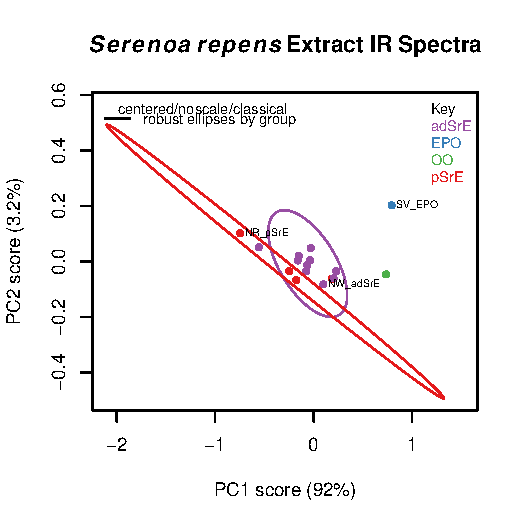
\includegraphics{/Users/bryanhanson/Documents/Professional/Research/R_Pkgs/ChemoSpec/docs/articles/ChemoSpec_files/figure-latex/Chunk10a-1} 

}

\caption{\label{classPCA}Classical PCA scores.}\label{fig:Chunk10a}
\end{figure}

\begin{Shaded}
\begin{Highlighting}[]
\NormalTok{r\_res <{-}}\StringTok{ }\KeywordTok{r\_pcaSpectra}\NormalTok{(SrE3.IR,}
  \DataTypeTok{choice =} \StringTok{"noscale"}\NormalTok{)}
\KeywordTok{plotScores}\NormalTok{(SrE3.IR, r\_res,}
  \DataTypeTok{main =}\NormalTok{ myt,}
  \DataTypeTok{pcs =} \KeywordTok{c}\NormalTok{(}\DecValTok{1}\NormalTok{,}\DecValTok{2}\NormalTok{),}
  \DataTypeTok{ellipse =} \StringTok{"rob"}\NormalTok{,}
  \DataTypeTok{tol =} \FloatTok{0.01}\NormalTok{)}
\end{Highlighting}
\end{Shaded}

\begin{ShadedResult}
\begin{verbatim}
#  Group EPO
#   has only 1 member (no ellipse possible)
\end{verbatim}
\end{ShadedResult}
\begin{ShadedResult}
\begin{verbatim}
#  Group OO
#   has only 1 member (no ellipse possible)
\end{verbatim}
\end{ShadedResult}
\begin{figure}

{\centering 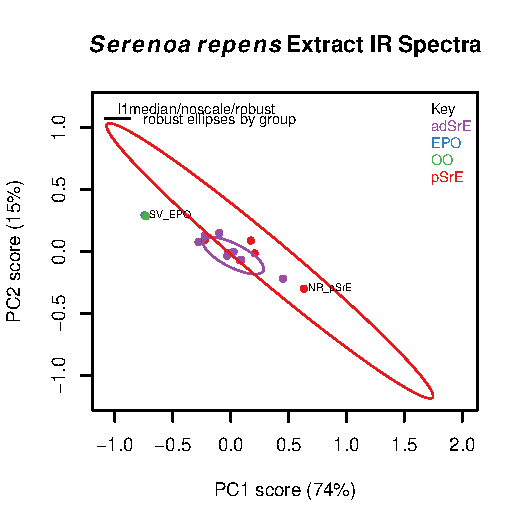
\includegraphics{/Users/bryanhanson/Documents/Professional/Research/R_Pkgs/ChemoSpec/docs/articles/ChemoSpec_files/figure-latex/Chunk21-1} 

}

\caption{\label{robPCA}Robust PCA scores.}\label{fig:Chunk21}
\end{figure}

Plots such as shown in Figures \ref{classPCA} and \ref{robPCA} can give
you an idea of potential outliers, but \texttt{ChemoSpec} includes more
sophisticated approaches. The function \texttt{pcaDiag} can produce two
types of plots that can be helpful (Figures \ref{OD} and \ref{SD}). The
meaning and interpretation of these plots is discussed in more detail in
Varmuza and Filzmoser, Chapter 3 \citep{Filzmoser2009}.

\begin{Shaded}
\begin{Highlighting}[]
\NormalTok{diagnostics <{-}}\StringTok{ }\KeywordTok{pcaDiag}\NormalTok{(SrE3.IR, c\_res,}
  \DataTypeTok{pcs =} \DecValTok{2}\NormalTok{,}
  \DataTypeTok{plot =} \StringTok{"OD"}\NormalTok{)}
\end{Highlighting}
\end{Shaded}

\begin{figure}

{\centering 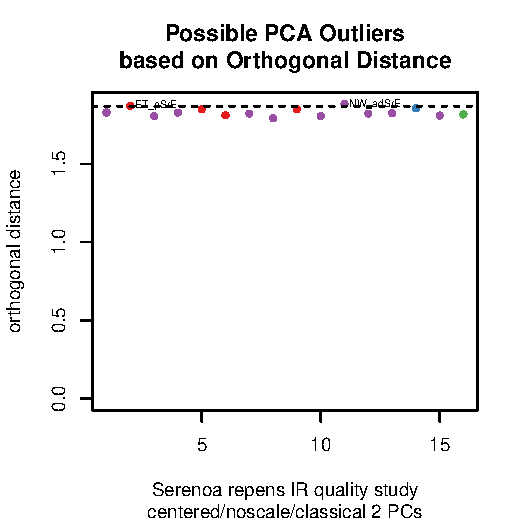
\includegraphics{/Users/bryanhanson/Documents/Professional/Research/R_Pkgs/ChemoSpec/docs/articles/ChemoSpec_files/figure-latex/Chunk22-1} 

}

\caption{\label{OD}Diagnostics: orthogonal distances.}\label{fig:Chunk22}
\end{figure}

\begin{Shaded}
\begin{Highlighting}[]
\NormalTok{diagnostics <{-}}\StringTok{ }\KeywordTok{pcaDiag}\NormalTok{(SrE3.IR, c\_res,}
  \DataTypeTok{pcs =} \DecValTok{2}\NormalTok{,}
  \DataTypeTok{plot =} \StringTok{"SD"}\NormalTok{)}
\end{Highlighting}
\end{Shaded}

\begin{figure}

{\centering 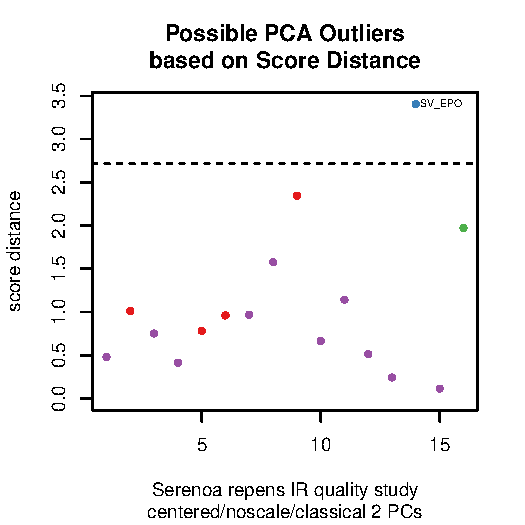
\includegraphics{/Users/bryanhanson/Documents/Professional/Research/R_Pkgs/ChemoSpec/docs/articles/ChemoSpec_files/figure-latex/Chunk23-1} 

}

\caption{\label{SD}Diagnostics: score distances.}\label{fig:Chunk23}
\end{figure}

Depending upon your data, and your interpretation of the results, you
may decide that some samples should be discarded, in which case you can
use \texttt{removeSample} as previously described, then repeat the PCA
analysis. The next step for most people is to determine the number of
PCs needed to describe the data. This is usually done with a scree plot
as shown in Figure \ref{scree}. \texttt{ChemoSpec} has an alternate
style scree plot which I actually think is much more informative (Figure
\ref{scree2}).

If you are using classical PCA, you can also get a sense of the number
of PCs needed via a bootstrap method, as shown in Figure \ref{boot}.
Note that this method is iterative and takes a bit of time. Comparing
these results to the scree plots, you'll see that the bootstrap method
suggests that 4 or 5 PCs would not always be enough to reach the 95\%
level, while the scree plots suggest that 2 PC are sufficient.

\begin{Shaded}
\begin{Highlighting}[]
\KeywordTok{plotScree}\NormalTok{(c\_res, }\DataTypeTok{main =}\NormalTok{ myt)}
\end{Highlighting}
\end{Shaded}

\begin{figure}

{\centering 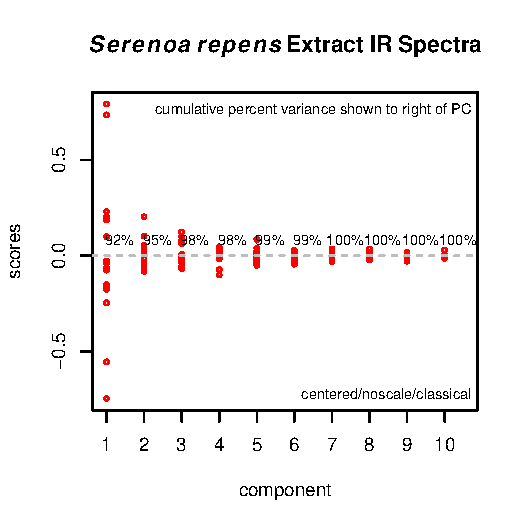
\includegraphics{/Users/bryanhanson/Documents/Professional/Research/R_Pkgs/ChemoSpec/docs/articles/ChemoSpec_files/figure-latex/Chunk24-1} 

}

\caption{\label{scree}Scree plot.}\label{fig:Chunk24}
\end{figure}

\begin{Shaded}
\begin{Highlighting}[]
\KeywordTok{plotScree}\NormalTok{(c\_res, }\DataTypeTok{style =} \StringTok{"alt"}\NormalTok{, }\DataTypeTok{main =}\NormalTok{ myt)}
\end{Highlighting}
\end{Shaded}

\begin{figure}

{\centering 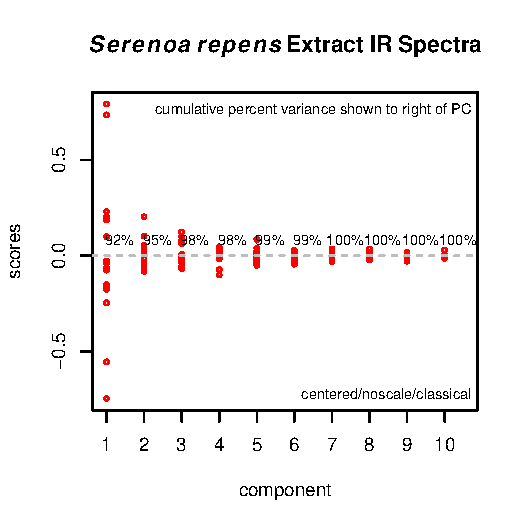
\includegraphics{/Users/bryanhanson/Documents/Professional/Research/R_Pkgs/ChemoSpec/docs/articles/ChemoSpec_files/figure-latex/Chunk24a-1} 

}

\caption{\label{scree2}Alternate style scree plot.}\label{fig:Chunk24a}
\end{figure}

\begin{Shaded}
\begin{Highlighting}[]
\NormalTok{out <{-}}\StringTok{ }\KeywordTok{cv\_pcaSpectra}\NormalTok{(SrE3.IR,}
  \DataTypeTok{pcs =} \DecValTok{5}\NormalTok{)}
\end{Highlighting}
\end{Shaded}

\begin{figure}

{\centering 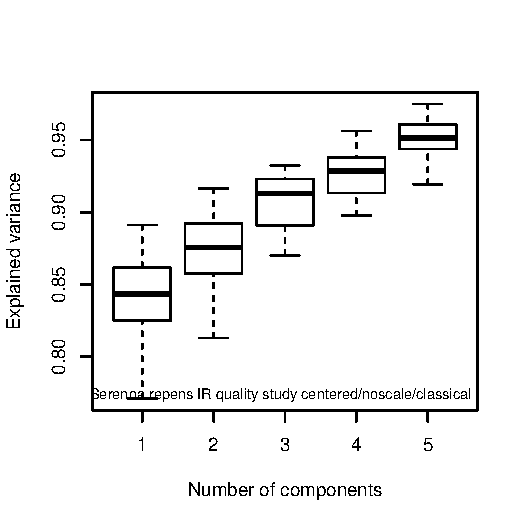
\includegraphics{/Users/bryanhanson/Documents/Professional/Research/R_Pkgs/ChemoSpec/docs/articles/ChemoSpec_files/figure-latex/Chunk25-1} 

}

\caption{\label{boot}Bootstrap analysis for no. of principal components.}\label{fig:Chunk25}
\end{figure}

Now let's turn to viewing scores in 3D. There are currently two options
in \texttt{ChemoSpec}: plotting using \texttt{lattice} graphics, which
produces a static plot that you have to adjust manually, and an
interactive plot based on package \texttt{rgl}. Probably the best place
to start is with \texttt{plotScoresRGL}. It it well suited to exploring
data, and can be printed out in high quality. However, the nature of the
\texttt{openGL} graphics device means that the title and the legend move
with the data, so this may not give a hardcopy suitable for
publications. This interactive plot cannot be invoked in this document,
but here are the necessary commands:

\begin{Shaded}
\begin{Highlighting}[]
\KeywordTok{plotScoresRGL}\NormalTok{(SrE3.IR, c\_res,}
  \DataTypeTok{main =} \StringTok{"S. repens IR Spectra"}\NormalTok{,}
  \DataTypeTok{leg.pos =} \StringTok{"A"}\NormalTok{,}
  \DataTypeTok{t.pos =} \StringTok{"B"}\NormalTok{) }\CommentTok{\# not run {-} it\textquotesingle{}s interactive!}
\end{Highlighting}
\end{Shaded}

For full details, of course take a look at the manual page,
\texttt{?plotScoresRGL}. If you want a similar and probably more
publication-worthy plot, you can use \texttt{plotScores3D} as shown in
Figure \ref{s3D}. In this example we've set \texttt{ellipse = FALSE}
because the ``adSrE'' data points form a very elongated ellipse which
forces the plotting limits in such a way that other points become very
hard to see.

\begin{Shaded}
\begin{Highlighting}[]
\KeywordTok{plotScores3D}\NormalTok{(SrE3.IR, c\_res,}
  \DataTypeTok{main =}\NormalTok{ myt,}
  \DataTypeTok{ellipse =} \OtherTok{FALSE}\NormalTok{)}
\end{Highlighting}
\end{Shaded}

\begin{figure}

{\centering 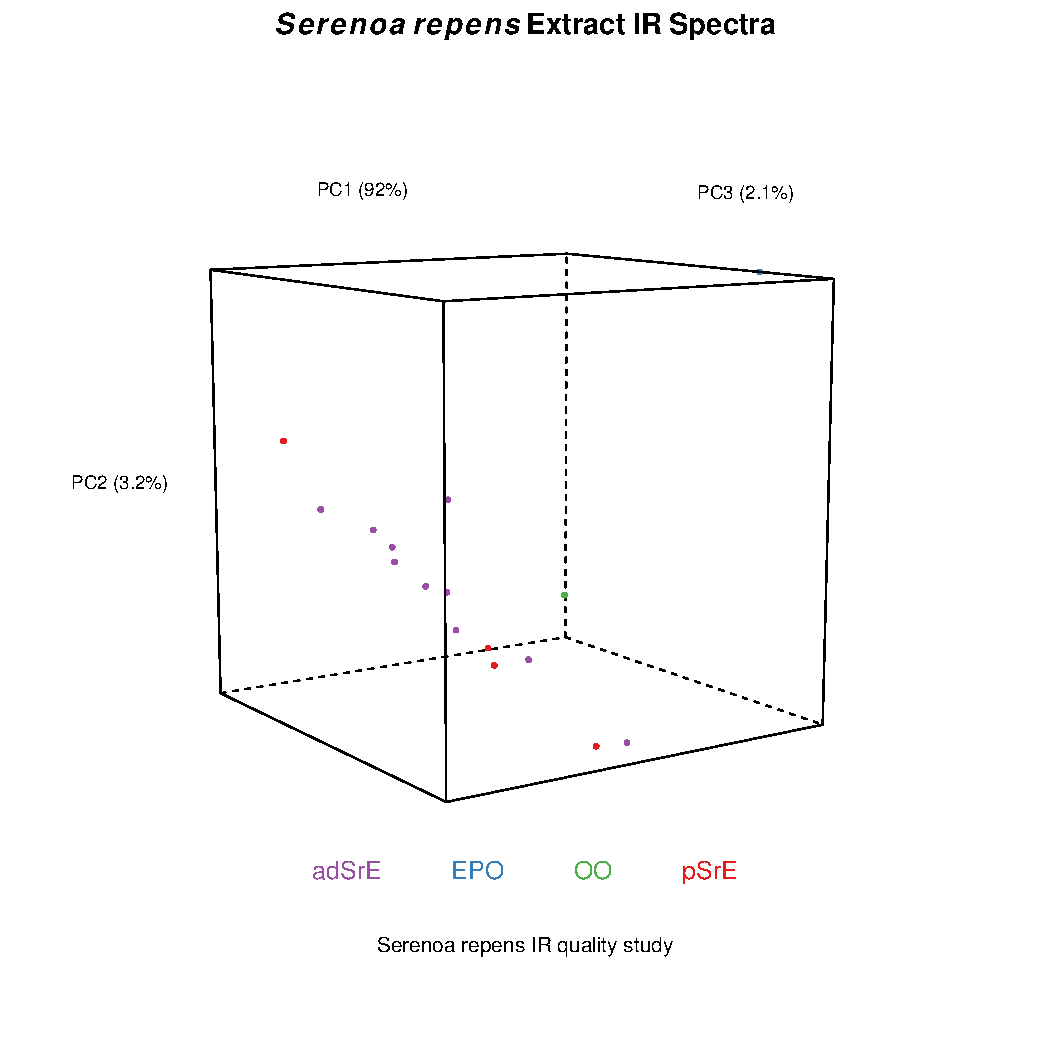
\includegraphics[width=\linewidth,height=\linewidth]{/Users/bryanhanson/Documents/Professional/Research/R_Pkgs/ChemoSpec/docs/articles/ChemoSpec_files/figure-latex/Chunk27-1} 

}

\caption{\label{s3D}Plotting scores in 3D using plotScores3D.}\label{fig:Chunk27}
\end{figure}

In addition to the scores, PCA also produces loadings which tell you how
each variable (frequencies in spectral applications) affect the scores.
Examining these loadings can be critical to interpreting your results.
Figure \ref{load} gives an example. You can see that the different
carbonyl peaks have a large and opposing effect on PC 1. PC 2 on the
other hand is driven by a number of peaks, with some interesting
opposing peaks in the hydrocarbon region. While the actual analysis of
the data is not our goal here, it would appear that PC 1 is sensitive to
the ester vs.~acid carbonyl group, and PC 2 is detecting the saturated
vs.~unsaturated fatty acid chains (the latter having
\(\mathsf{C_{sp2}-H}\) peaks).

\begin{Shaded}
\begin{Highlighting}[]
\KeywordTok{plotLoadings}\NormalTok{(SrE3.IR, c\_res,}
  \DataTypeTok{main =}\NormalTok{ myt,}
  \DataTypeTok{loads =} \KeywordTok{c}\NormalTok{(}\DecValTok{1}\NormalTok{, }\DecValTok{2}\NormalTok{),}
  \DataTypeTok{ref =} \DecValTok{1}\NormalTok{)}
\end{Highlighting}
\end{Shaded}

\begin{figure}

{\centering 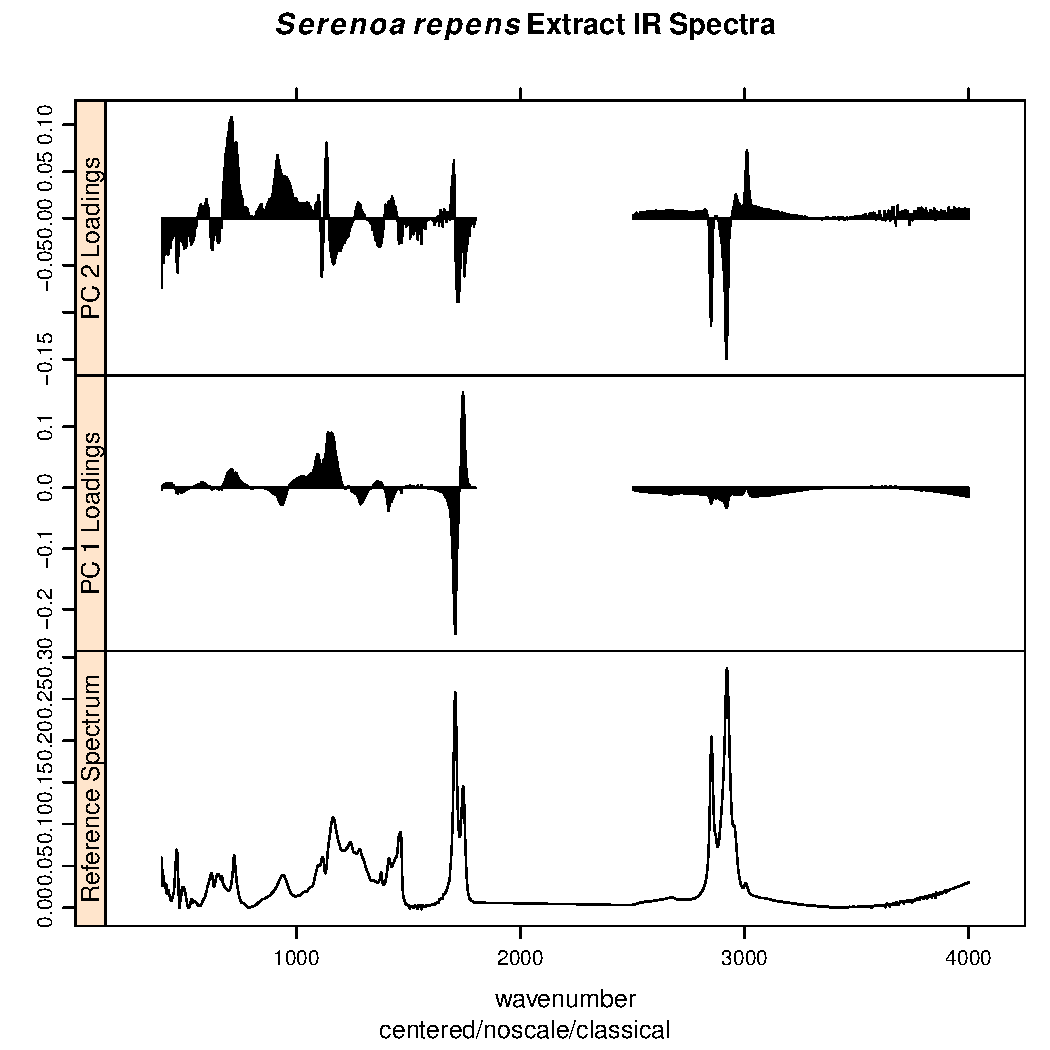
\includegraphics[width=\linewidth,height=\linewidth]{/Users/bryanhanson/Documents/Professional/Research/R_Pkgs/ChemoSpec/docs/articles/ChemoSpec_files/figure-latex/Chunk29-1} 

}

\caption{\label{load}Loading plot.}\label{fig:Chunk29}
\end{figure}

You can also plot one loading against another, using function
\texttt{plot2Loadings} (Figure \ref{load2}). This is typically not too
useful for spectroscopic data, since many of the variables are
correlated (as they are parts of the same peak, hence the serpentine
lines in the figure). The most extreme points on the plot, however, can
give you an idea of which peaks (frequencies) serve to differentiate a
pair of PCs, and hence, drive your data clustering.

\begin{Shaded}
\begin{Highlighting}[]
\NormalTok{res <{-}}\StringTok{ }\KeywordTok{plot2Loadings}\NormalTok{(SrE3.IR, c\_res,}
  \DataTypeTok{main =}\NormalTok{ myt,}
  \DataTypeTok{loads =} \KeywordTok{c}\NormalTok{(}\DecValTok{1}\NormalTok{, }\DecValTok{2}\NormalTok{),}
  \DataTypeTok{tol =} \FloatTok{0.002}\NormalTok{)}
\end{Highlighting}
\end{Shaded}

\begin{figure}

{\centering 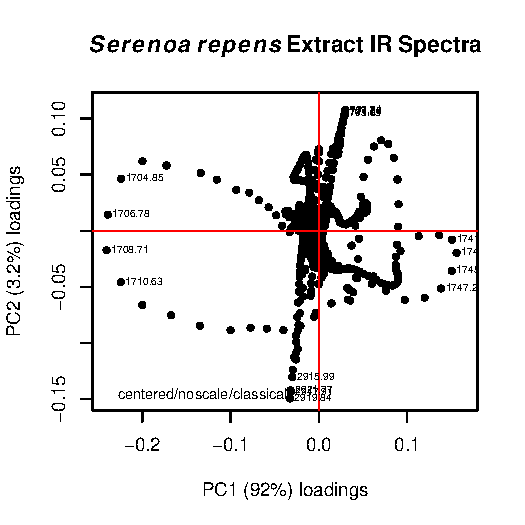
\includegraphics{/Users/bryanhanson/Documents/Professional/Research/R_Pkgs/ChemoSpec/docs/articles/ChemoSpec_files/figure-latex/Chunk30-1} 

}

\caption{\label{load2}Plotting one loading vs. another.}\label{fig:Chunk30}
\end{figure}

However, a potentially more useful approach is to use an s-plot to
determine which variables have the greatest influence. A standard
loadings plot (\texttt{plotLoadings}) shows you which frequency ranges
contribute to which principal components, but the plot allows the
vertical axis to be free. Unless you look at the y axis scale, you get
the impression that the loadings for principal component 1 etc. all
contribute equally. The function \texttt{sPlotSpectra} plots the
correlation of each frequency variable with a particular score against
the covariance of that frequency variable with the same score. The
result is an s-shaped plot with the most influential frequency variables
in the upper right hand and lower left quadrants. An example is shown in
Figure \ref{splot} with a detail view in Figure \ref{splot2}. In the
latter figure you can clearly see the influence of the carbonyl peaks.
This method was reported in\cite{Wiklund2008}.

\begin{Shaded}
\begin{Highlighting}[]
\NormalTok{spt <{-}}\StringTok{ }\KeywordTok{sPlotSpectra}\NormalTok{(SrE3.IR, c\_res,}
  \DataTypeTok{main =}\NormalTok{ myt,}
  \DataTypeTok{pc =} \DecValTok{1}\NormalTok{,}
  \DataTypeTok{tol =} \FloatTok{0.001}\NormalTok{)}
\end{Highlighting}
\end{Shaded}

\begin{figure}

{\centering 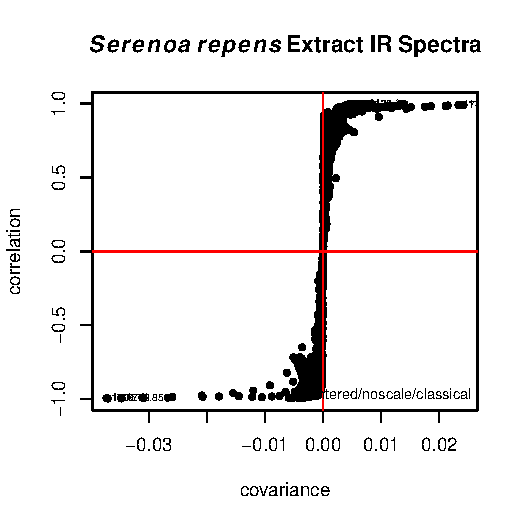
\includegraphics{/Users/bryanhanson/Documents/Professional/Research/R_Pkgs/ChemoSpec/docs/articles/ChemoSpec_files/figure-latex/Chunk30a-1} 

}

\caption{\label{splot}s-Plot to identify influential frequencies.}\label{fig:Chunk30a}
\end{figure}

\begin{Shaded}
\begin{Highlighting}[]
\NormalTok{spt <{-}}\StringTok{ }\KeywordTok{sPlotSpectra}\NormalTok{(SrE3.IR, c\_res,}
  \DataTypeTok{main =} \StringTok{"Detail of s{-}Plot"}\NormalTok{,}
  \DataTypeTok{pc =} \DecValTok{1}\NormalTok{,}
  \DataTypeTok{tol =} \FloatTok{0.05}\NormalTok{,}
  \DataTypeTok{xlim =} \KeywordTok{c}\NormalTok{(}\OperatorTok{{-}}\FloatTok{0.04}\NormalTok{, }\FloatTok{{-}0.01}\NormalTok{),}
  \DataTypeTok{ylim =} \KeywordTok{c}\NormalTok{(}\OperatorTok{{-}}\FloatTok{1.05}\NormalTok{, }\FloatTok{{-}0.9}\NormalTok{))}
\end{Highlighting}
\end{Shaded}

\begin{figure}

{\centering 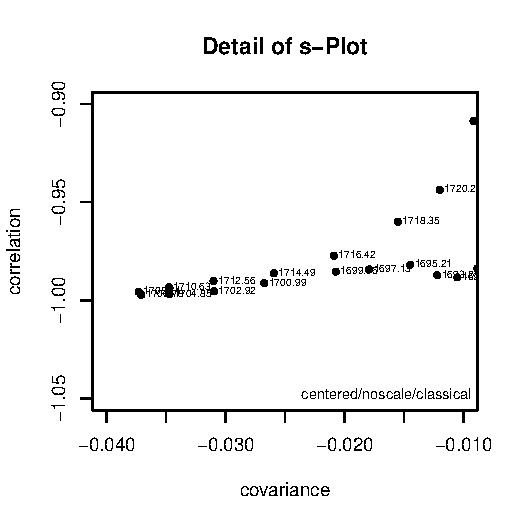
\includegraphics{/Users/bryanhanson/Documents/Professional/Research/R_Pkgs/ChemoSpec/docs/articles/ChemoSpec_files/figure-latex/Chunk30b-1} 

}

\caption{\label{splot2}s-Plot detail.}\label{fig:Chunk30b}
\end{figure}

Finally, you can blend the ideas of PCA and HCA. Since PCA eliminates
the noise in a data set (after you have selected the important PCs), you
can carry out HCA on the PCA scores, as now the scores represent the
cleaned up data. The result using the \texttt{SrE.IR} data set are not
different than doing HCA on the raw spectra, so we won't illustrate it,
but the command would be:

\begin{Shaded}
\begin{Highlighting}[]
\KeywordTok{hcaScores}\NormalTok{(SrE3.IR,  c\_res,}
  \DataTypeTok{scores =} \KeywordTok{c}\NormalTok{(}\DecValTok{1}\OperatorTok{:}\DecValTok{5}\NormalTok{),}
  \DataTypeTok{main =}\NormalTok{ myt)}
\end{Highlighting}
\end{Shaded}

\hypertarget{anova-pca}{%
\subsection{ANOVA-PCA}\label{anova-pca}}

Harrington \emph{et. al.}\citep{Harrington2005} (and a few others --
\cite{Pinto2008}) have demonstrated a method which combines traditional
ANOVA with PCA. Standard PCA is blind to class membership, though one
generally colors the points in a score plot using the known class
membership. ANOVA-PCA uses the class membership to divide the original
centered data matrix into submatrices. Each submatrix corresponds to a
particular factor, and the rows of the submatrix have been replaced by
the average spectrum of each level of the factor. The original data set
is thought of as a sum of these submatrices plus residual error. The
residual error is added back to each submatrix and then PCA is
performed. This is conceptually illustrated in Figures \ref{aovPCA2} and
\ref{aovPCA1}.

\begin{figure}
\begin{center}
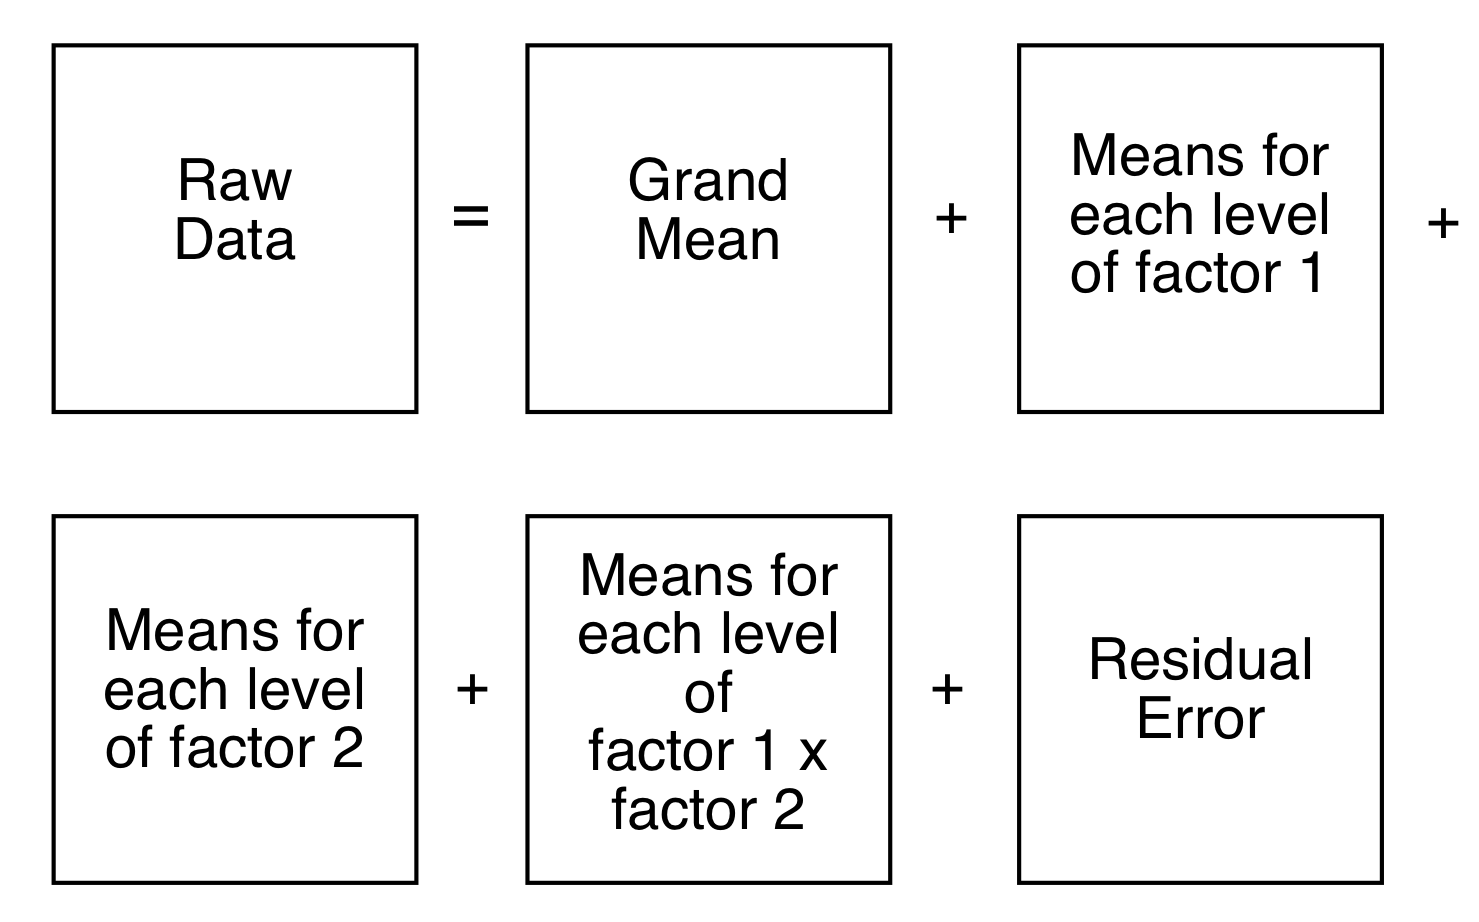
\includegraphics[scale = 0.5]{aovPCA2}
\caption{\label{aovPCA2}aovPCA breaks the data into a series of submatrices.}
\end{center}
\end{figure}

\begin{figure}
\begin{center}
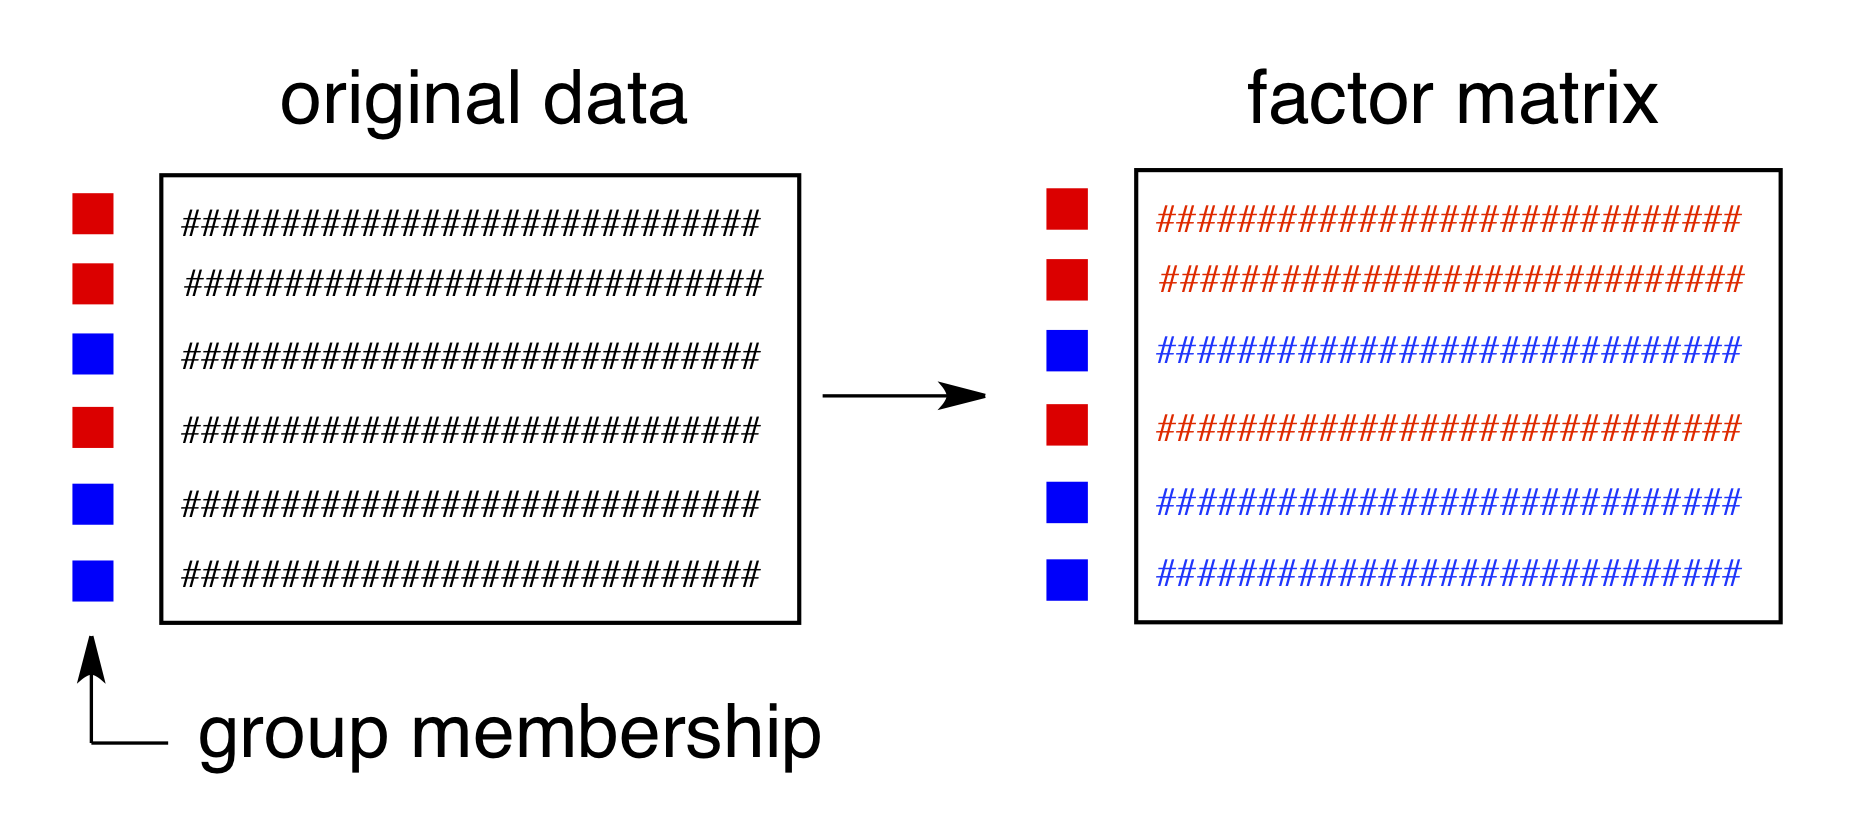
\includegraphics[scale = 0.6]{aovPCA1}
\caption{\label{aovPCA1}Submatrices are composed of rows which are averages of each factor level.}
\end{center}
\end{figure}

ANOVA-PCA has been implemented in \texttt{ChemoSpec} via the functions
\texttt{aov\_pcaSpectra}, \texttt{aovPCAscores} and
\texttt{aovPCAloadings}.\footnote{These functions were authored by Matt J. Keinsley.}
The idea here is that if a factor is significant, there will be
separation along PC1 in a plot of PC1 vs PC2. There are not enough
groups and levels within the \texttt{SrE.IR} data set to carry out
ANOVA-PCA. However, the help page for \texttt{aov\_pcaSpectra} contains
an example using the \texttt{CuticleIR} data set which illustrates how
to carry out the analysis. It also demonstrates another useful function,
\texttt{splitSpectraGroups} which allows you to take an existing group
designation and split it into new designations. See
\texttt{\textsl{?aov\_pcaSpectra}}.

\hypertarget{model-based-clustering-using-mclust}{%
\subsection{Model-Based Clustering Using
mclust}\label{model-based-clustering-using-mclust}}

PCA and HCA are techniques which are unsupervised and assume no
underlying model. HCA computes distances between pairs of spectra and
groups these in an iterative fashion until the dendrogram is complete.
PCA seeks out components that maximize the variance. While in PCA one
often (and \texttt{ChemoSpec} does) displays the samples coded by their
group membership, this information is not actually used in PCA; any
apparent correspondence between the sample group classification and the
clusters found is accidental in terms of the computation, but of course,
this is what one hopes to find!

\texttt{mclust} is a model-based clustering package that takes a
different approach.\citep{Scrucca2017}. \texttt{mclust} assumes that
there are groups within your data set, and that those groups are
multivariate normally distributed. Using an iterative approach,
\texttt{mclust} samples various possible groupings within your data set,
and uses a Bayesian Information Criterion (BIC) to determine which of
the various groupings it finds best fits the data distribution.
\texttt{mclust} looks for groups that follow certain constraints, for
instance, one constraint is that all the groups found must have a
spherical distribution of data points, while another allows for
ellipsoidal distributions. See the paper by Scrucca and Raftery
\citep{Scrucca2017} for more details. The basic idea however is that
\texttt{mclust} goes looking for groups in your data set, and then you
can compare the groupings it finds with the groupings you know to be
true.

\texttt{ChemoSpec} contains several functions that interface with and
extend \texttt{mclust} functions. \texttt{mclust} first uses the BIC to
determine which model best fits your data; these results are shown in
Figure \ref{mclust1}. Next, Figure \ref{mclust2} shows the groups that
\texttt{mclust} finds in the data. It's of some interest to visually
compare the score plot in Figure \ref{classPCA} with the \texttt{mclust}
results in Figure \ref{mclust2}. It looks like \texttt{mclust} groups
the two outliers with some of the rest of the data. Next,
\texttt{mclust} will map the true groups onto the groups it has found.
Points in error are X-ed out. These results can be seen in Figure
\ref{mclust3}. From this plot, you can see that \texttt{mclust} hasn't
done too well with this data set. In general, you have to be very
careful about using \texttt{mclust}'s notion of an error: it is very
hard to map the found groups onto the ``truth'' in an algorithmic way. I
lean toward not using the ``truth'' option in \texttt{mclust} more and
more.

\begin{Shaded}
\begin{Highlighting}[]
\NormalTok{model <{-}}\StringTok{ }\KeywordTok{mclustSpectra}\NormalTok{(SrE3.IR, c\_res,}
  \DataTypeTok{plot =} \StringTok{"BIC"}\NormalTok{,}
  \DataTypeTok{main =}\NormalTok{ myt)}
\end{Highlighting}
\end{Shaded}

\begin{figure}

{\centering 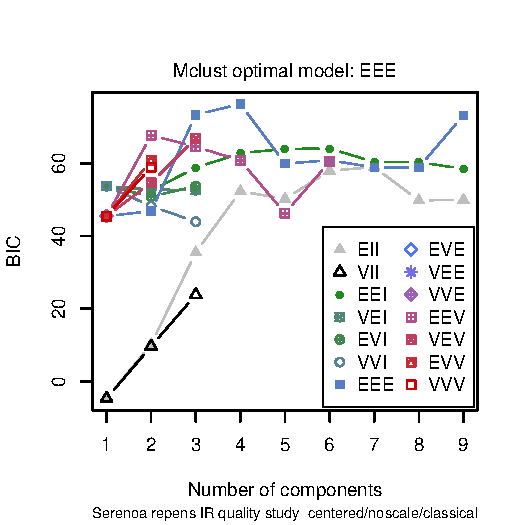
\includegraphics{/Users/bryanhanson/Documents/Professional/Research/R_Pkgs/ChemoSpec/docs/articles/ChemoSpec_files/figure-latex/Chunk35-1} 

}

\caption{\label{mclust1}mclust chooses an optimal model.}\label{fig:Chunk35}
\end{figure}

\begin{Shaded}
\begin{Highlighting}[]
\NormalTok{model <{-}}\StringTok{ }\KeywordTok{mclustSpectra}\NormalTok{(SrE3.IR, c\_res,}
  \DataTypeTok{plot =} \StringTok{"proj"}\NormalTok{,}
  \DataTypeTok{main =}\NormalTok{ myt)}
\end{Highlighting}
\end{Shaded}

\begin{figure}

{\centering 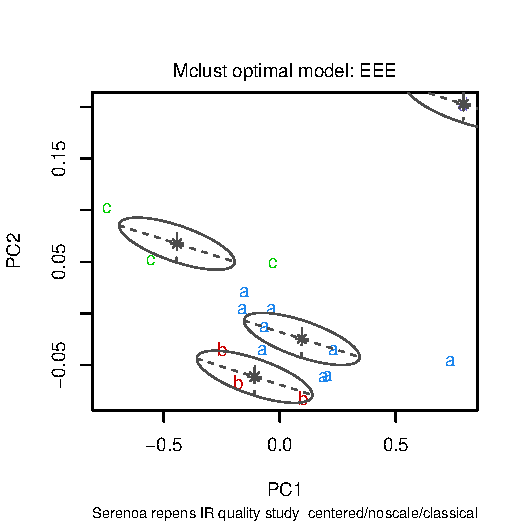
\includegraphics{/Users/bryanhanson/Documents/Professional/Research/R_Pkgs/ChemoSpec/docs/articles/ChemoSpec_files/figure-latex/Chunk36-1} 

}

\caption{\label{mclust2}mclust's thoughts on the matter.}\label{fig:Chunk36}
\end{figure}

\begin{Shaded}
\begin{Highlighting}[]
\NormalTok{model <{-}}\StringTok{ }\KeywordTok{mclustSpectra}\NormalTok{(SrE3.IR, c\_res,}
  \DataTypeTok{plot =} \StringTok{"errors"}\NormalTok{,}
  \DataTypeTok{main =}\NormalTok{ myt,}
  \DataTypeTok{truth =}\NormalTok{ SrE3.IR}\OperatorTok{$}\NormalTok{groups)}
\end{Highlighting}
\end{Shaded}

\begin{figure}

{\centering 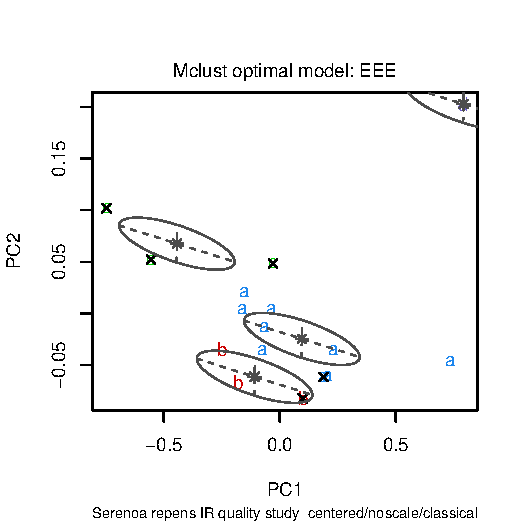
\includegraphics{/Users/bryanhanson/Documents/Professional/Research/R_Pkgs/ChemoSpec/docs/articles/ChemoSpec_files/figure-latex/Chunk37-1} 

}

\caption{\label{mclust3}Comparing mclust results to the TRUTH.}\label{fig:Chunk37}
\end{figure}

You can also do a similar analysis in 3D, using
\texttt{mclust3dSpectra}. This function uses \texttt{mclust} to find the
groups, but then uses non-\texttt{mclust} functions to draw confidence
ellipses. This function uses \texttt{rgl} graphics so it cannot
demonstrated here, but the commands would be:

\begin{Shaded}
\begin{Highlighting}[]
\CommentTok{\# not run {-} it\textquotesingle{}s interactive!}
\KeywordTok{mclust3dSpectra}\NormalTok{(SrE3.IR, c\_res)}
\end{Highlighting}
\end{Shaded}

You have all the options here that you do with \texttt{plotScoresRGL},
namely, classical, robust or no ellipses, control of the ellipse
details, and labeling of extreme points.

I hope you have enjoyed this tour of the features of \texttt{ChemoSpec}!

\hypertarget{functions-that-are-not-discussed-here}{%
\section{Functions That Are Not Discussed
Here}\label{functions-that-are-not-discussed-here}}

See the help files of course \ldots

\begin{enumerate}
  \item \texttt{splitSpectraGroups}  A good example of its use can be found in \texttt{\textsl{?aov\_pcaSpectra}}.
  \item \texttt{hypTestScores}: Run anova on PCA scores.
  \item \texttt{hmapSpectra}: Plot a seriated heat map.
  \item \texttt{evalClusters}: Compare various clustering options.
  \item \texttt{sgfSpectra} Apply Savitzky-Golay filters.
  \item \texttt{plotSpectraDist} Plot the distance between each spectrum and a reference spectrum.

\end{enumerate}

\hypertarget{color-and-symbol-options}{%
\section{\texorpdfstring{Color and Symbol Options
\label{ColSym}}{Color and Symbol Options }}\label{color-and-symbol-options}}

In \texttt{ChemoSpec}, the user may use any color name/format known to
\texttt{R}. When importing data, \texttt{ChemoSpec} will choose colors
for you automatically if desired. However, depending upon your needs,
you may wish to choose colors yourself. the current color scheme of a
\texttt{Spectra} object may be determined using \texttt{sumSpectra} or
changed using \texttt{conColScheme}. A fuller discussion of color issues
can be found in \texttt{?colorSymbol}.

In addition to colors, \texttt{"Spectra"} objects also contain a list of
symbols, and alternative symbols. These are useful for plotting in black
and white, or when color-blind individuals will be viewing the plots.
The alternative symbols are simply lower-case letters, as these are
needed for \texttt{plotScoresRGL}, and other \texttt{rgl}-graphics
driven functions which cannot plot traditional symbols.

\hypertarget{related-packages}{%
\section{Related Packages}\label{related-packages}}

Several other packages exist which do some of the same tasks as
\texttt{ChemoSpec}, and do other things as well. The package closest in
functionality to \texttt{ChemoSpec} is \texttt{hyperSpec} written by my
friend and collaborator Claudia Belietes (these packages were developed
independently around the same time).\citep{Beleites2018} There is also a
package designed to interconvert \texttt{Spectra} objects and
\texttt{hyperSpec} objects, which allows one to move data between the
packages more easily \citep{HansonMcManus2018}. There is a lot
development going in the \texttt{R} ecosystem, and new packages appear
steadily (and sometimes they disappear!). A good place to check these
things out is the
\href{http://cran.at.r-project.org/web/views/ChemPhys.html}{Chemometrics and Computational Physics Task View}.

%\showmatmethods
\showacknow

\pnasbreak 

\bibliography{chemometrics.bib}
\bibliographystyle{jss}



\end{document}
